
\chapter{System Implementation}
\label{ch:impl}

In the previous chapter, the overall design requirements for developing an embodiment and body schema transfer system were specified. This chapter will discuss the implementation details for a designer friendly embodiment modeling framework. The major components for the framework are discussed here: the Meta-modeling editor, modalities information channels and meta-blocks, the integration with an existing game engine (Unity 3D), performance optimizations, and physical embodiment toolkit. 

\section{Embodiment Framework Overview}


\begin{figure}[b!]
\centering
\captionsetup{justification=centering} 
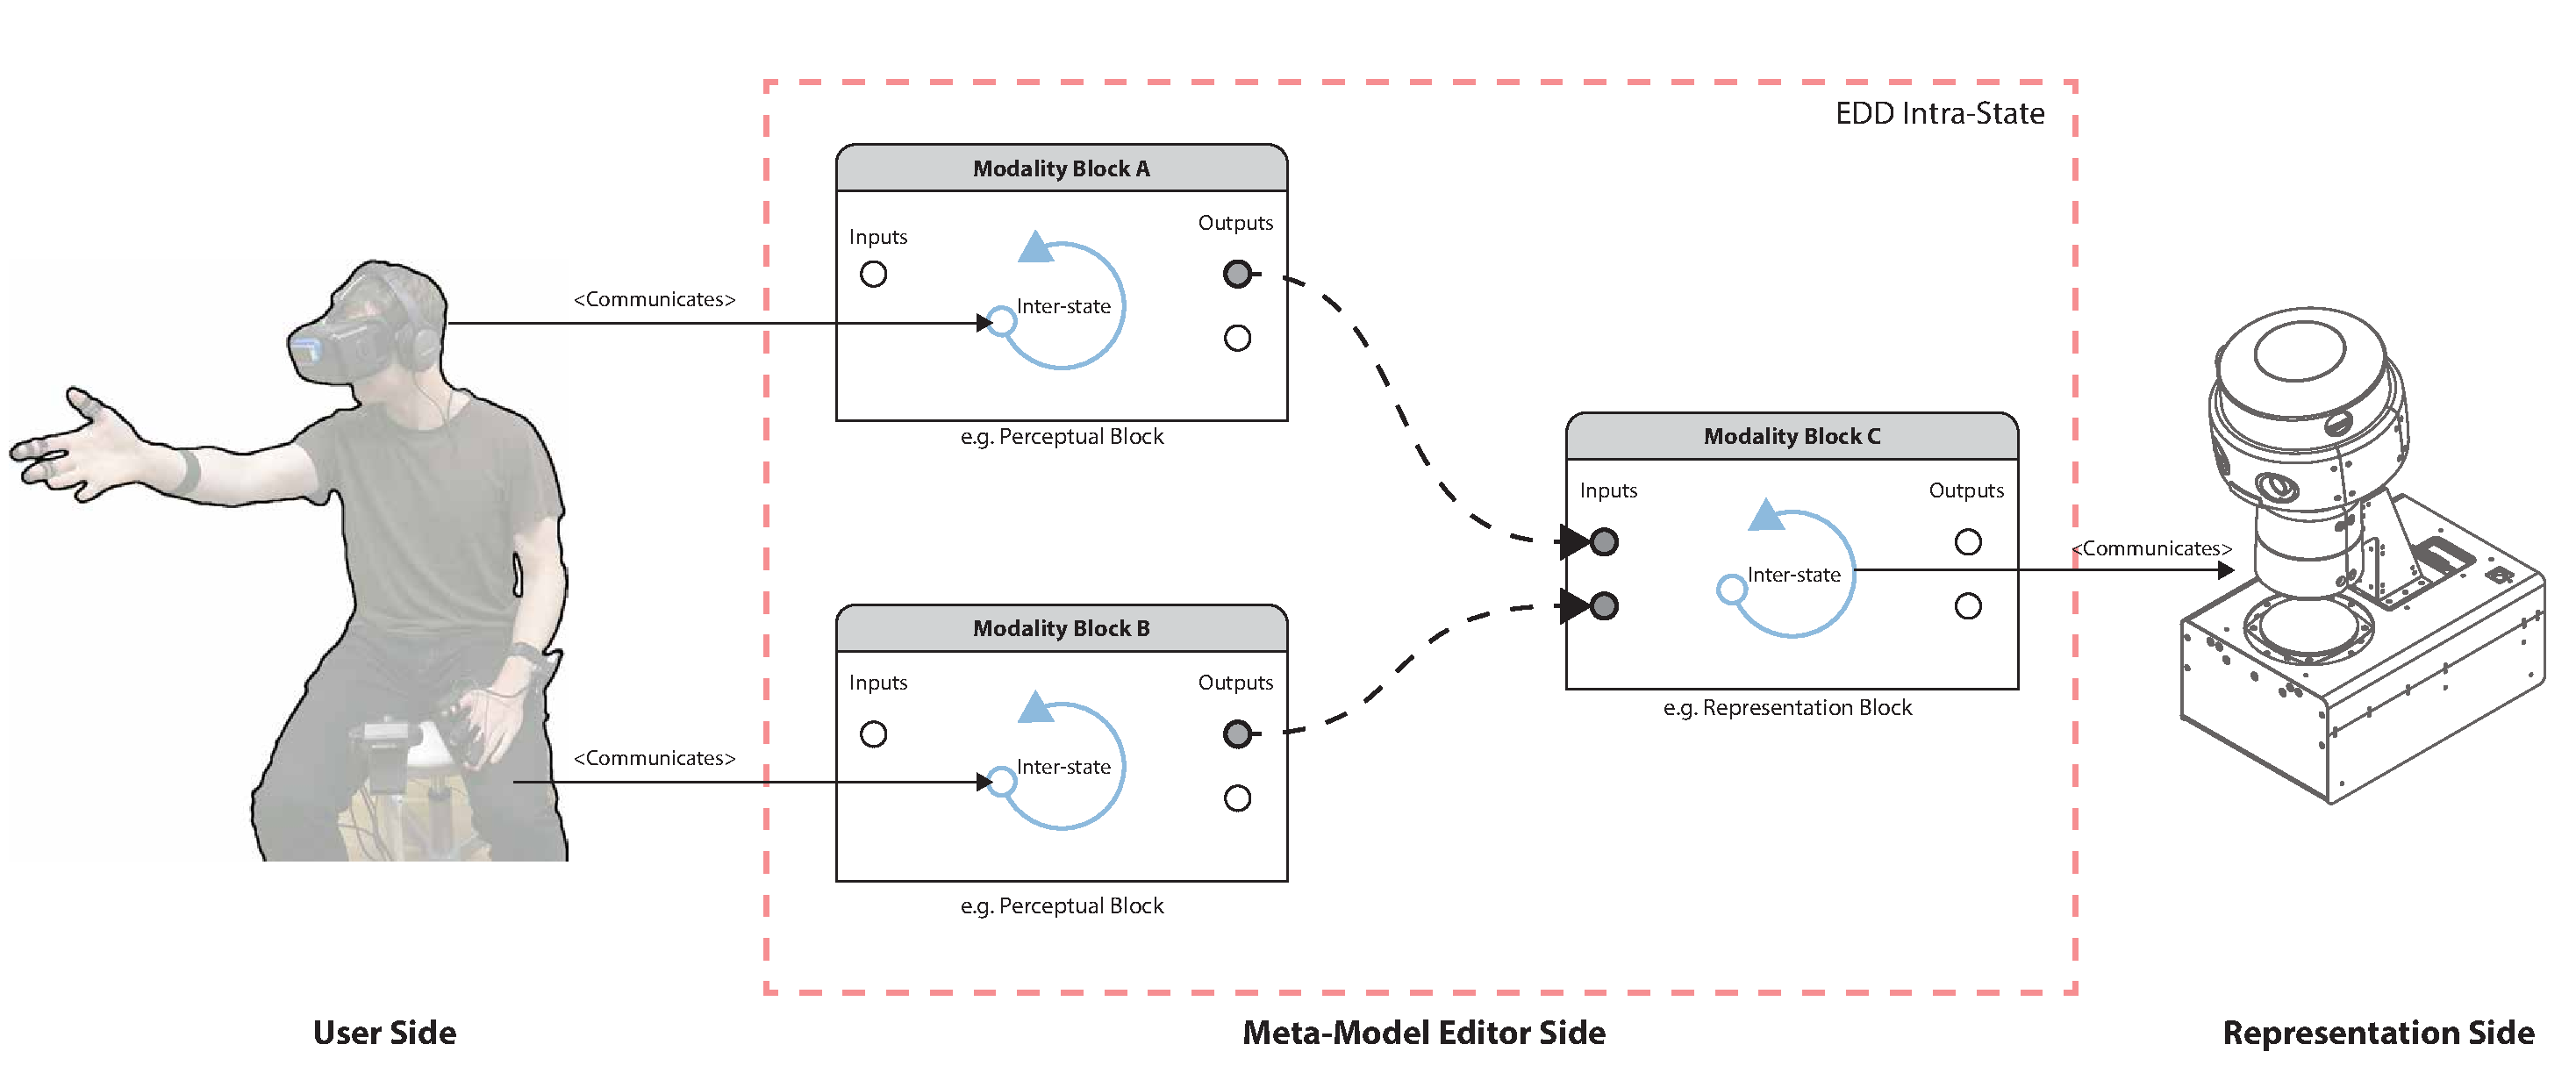
\includegraphics[width=1\textwidth]{figures/system/EDD_Editor_Overview.pdf}
\caption{An overview for Embodiment Framework components.}
  \label{fig:system-edd-overview}
\end{figure}

The embodiment framework contains various components and blocks that defines the topology of the system and representation. An overview of the framework is shown in \Figure{fig:system-edd-overview}. The framework consists of: \textbf{User side} which communicates the state of the operating user with the model using tracking and perceptual devices, \textbf{Meta-Model Editor side} which defines the interacting blocks and modules of the target schema of the system, and \textbf{Representation side} which communicates the state of the used representation (virtual or physical) with the model. 

The user side contains modular tracking and perceptual hardware in which it can be customized depending on the intended application. For visuals presentation to user's eyes, a head mounted display is mainly for presence transfer systems (derived from telexistence systems). For body tracking, several tracking systems has been integrated into the framework in order to assist the degree of body tracking based on the number of joints intended to be tracked. For example, when head tracking is only needed, then HMD built-in tracking functionality can be used without the need for an external tracker, but when eyes, arms or legs tracking was required, then different tracking approaches would be used (individually or combined, e.g. optical tracking and data gloves systems). The perceptual and tracking modalities are exposed into the meta-modeling editor as set of blocks that transfer the state of the modalities from/to the model. For example, a [HMD] block would have an input representing the images to be displayed, and an output for its spatial position and rotation. 

Representaiton side is dependant on the type of the body used in the representation. Two types of representations are addressed: Robotic representation, and virtual bodies. These representations can be used individually or in a combination, for example superimposing virtual arms on the visual feed from a remote robot representation. The representation blocks are responsible to communicate with the used body to transfer the modalities data channels from the meta-model and the representation. For postural modalities, joints data are used to control the position and orientation of the links used in the body (e.g. servo motor for robotic form). Similarly, sensory modalities uses transfer blocks to communicate the captured information flow from the representation to the meta-model. [Eyes] transfer block, for example, provides an image stream from the cameras used in the representation.


The meta-modeling editor handles the inter-states and intra-state of the modalities channels flow of the blocks used. The inter-state corresponds to the internal processes of the block throughout a procedure of capturing the inputs through the available slots, applying internal calculations or alteration to that input channels, and expose the results though output slots with a corresponding data type. The intra-state of the meta-model controls the flow of the channels, and constraints the data flow and types used. The intra-state is defined by the embodiment designer.


\section{Meta-Modeling Editor}

\begin{figure}[b!]
\centering
\captionsetup{justification=centering} 
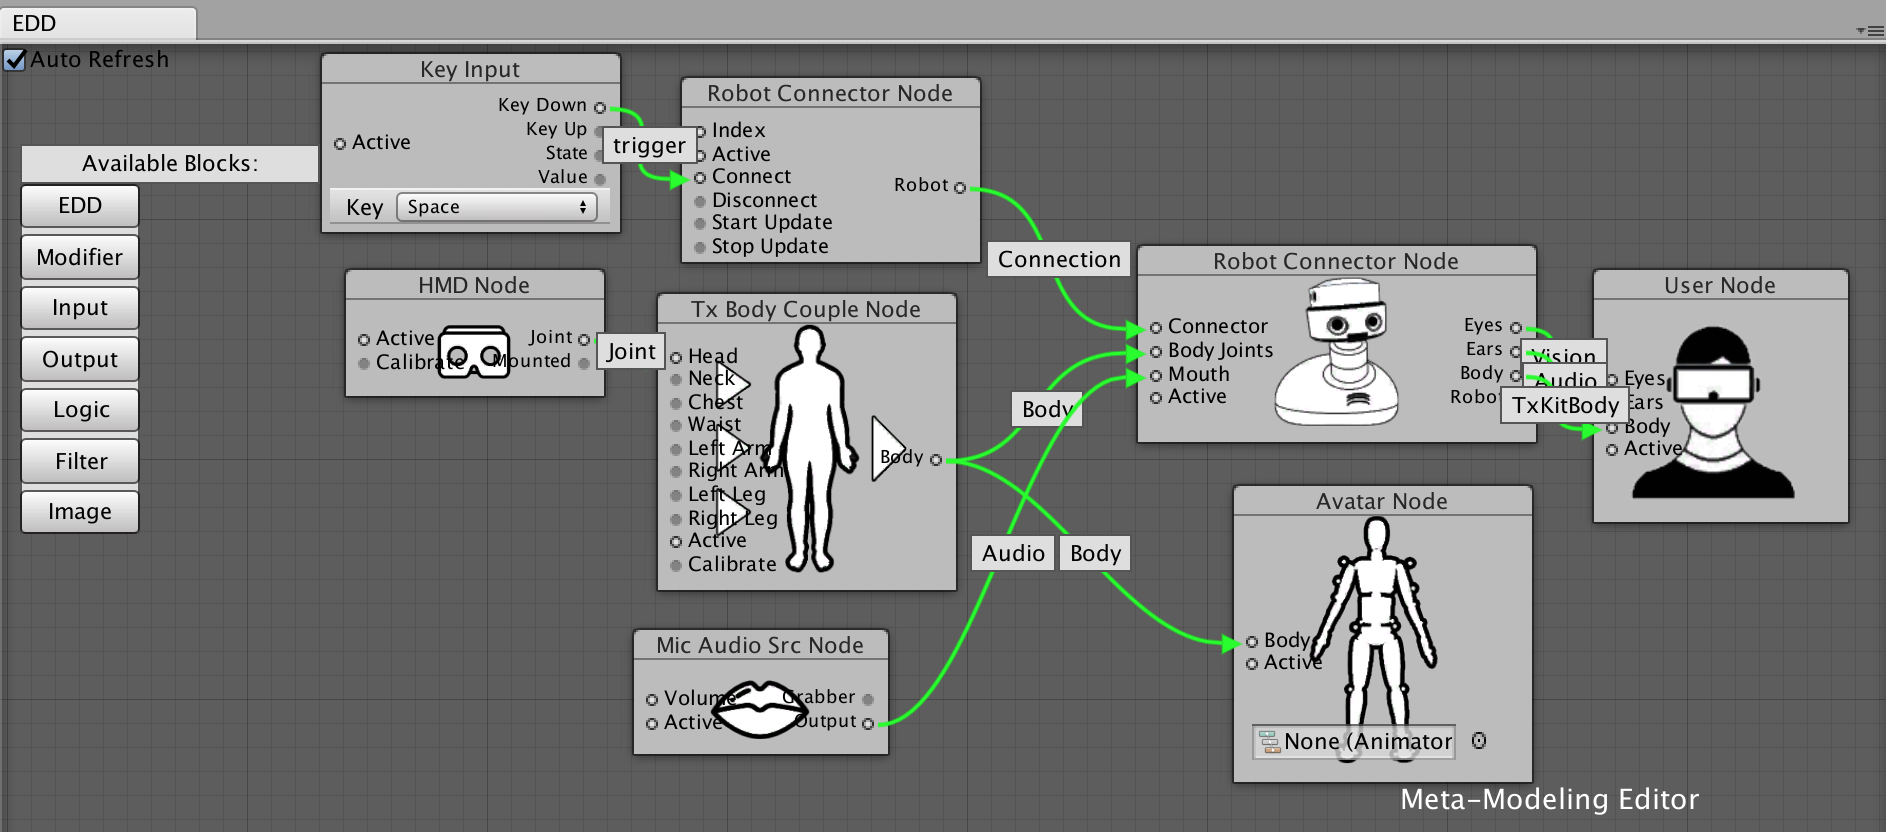
\includegraphics[width=1\textwidth]{figures/system/MetaEditor.png}
\caption{Meta-Modeling Editor Overview.}
  \label{fig:system-metaeditor}
\end{figure}

The meta-modeling editor provides a designer oriented approach to model the interactions between the user and the representation by using various types of meta-blocks. \Figure{fig:system-metaeditor} shows an overview of the meta-modeling editor developed in this thesis. This editor has been implemented under Unity3D. The reason of choosing this game engine in particular is that this engine has been widely accepted platform by both inexperienced and professional designers and programmers, also this engine supports cross-platform deployment which would increase the usability of the meta-modeler system. The design consideration for this editor is to focus on graphically oriented visual programming with minimum amount of writing code to create the model. The editor contains several categories of meta-blocks which can be basic arithmetic or geometric operation blocks, or higher level of interaction such as body tracking blocks. \Figure{fig:system-blocks-nodes} shows how the meta-blocks are organized in a tree structure based on the category and functionality. The designer can access the blocks directly from the side panel in a hierarchical structure, or directly search for the required block by using the search function (Ctrl+Mouse Click) and entering part of the block name in the search box. Using this mechanism, the designer would avoids the confusion of finding the required block. 

\begin{figure}[htpb]
\centering
\captionsetup{justification=centering} 
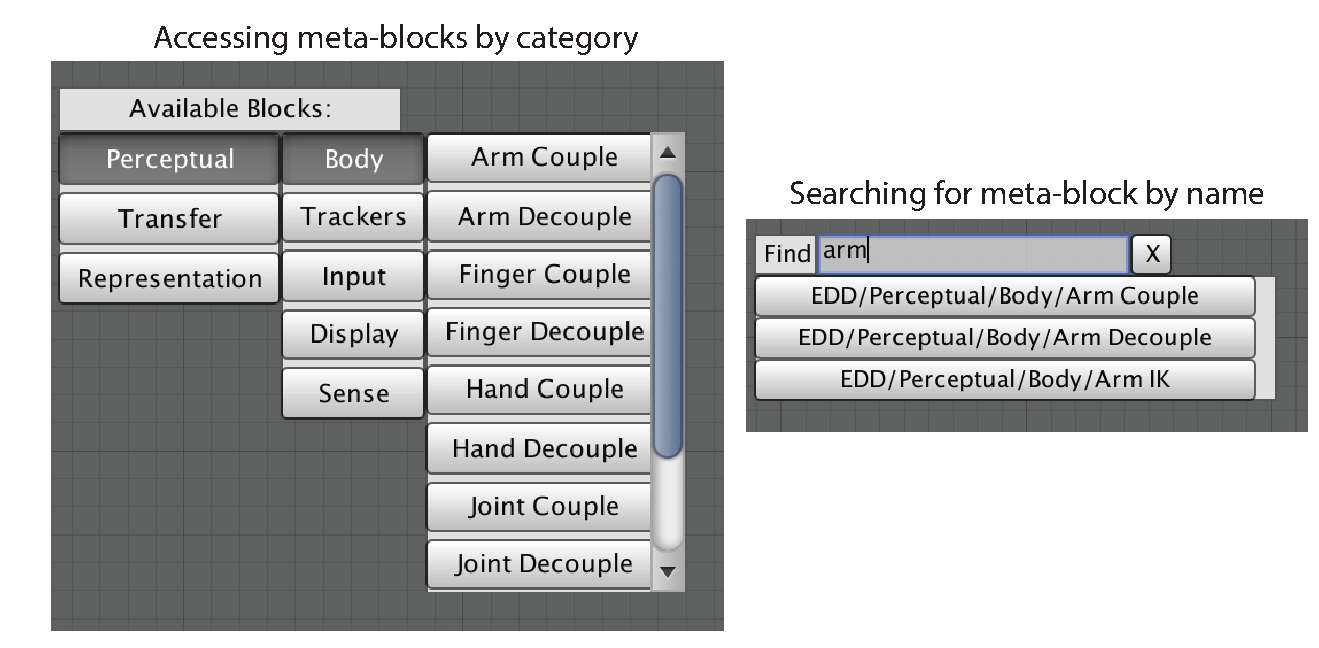
\includegraphics[width=0.8\textwidth]{figures/system/Blocks/Nodes.pdf}
\caption{Accessing meta-blocks by Searching or Category.}
  \label{fig:system-blocks-nodes}
\end{figure}

In order to use the meta-modeling editor, the designer needs to create a new [EDD Model] object under Unity3D editor by choosing: \textit{GameObject Menu \textrightarrow EDD Model}. Once an EDD Model is added, its possible to access the Meta-Modeling editor by selecting the model and clicking [Open Model] from the inspector. The Mea-Modeling editor supports to run multiple models on parallel, so its possible to design dedicate each model into different application or use case. For example one meta-model handles the auditory transmission and alteration, and another one for the body control and mapping. Thus the design process can be distributed.

When a meta-block is added to the model, the block exposes the available input and output channels (or slots) that provides the accessibility from/to its functionality. As a matter of making a convention, the data flow of the blocks always goes from left to right, so input slots are located on the left side, and output slots on the right. When more than one block is added to the model, its possible to connect their channels as long as the channel data matches. Although it constraints the modeling process, however it assists the designer to quickly understand which channels can be connected by highlighting the acceptable input channels in all the blocks added to the model. When channels are connected, a data flow is registered between them. \Figure{fig:system-blocks-flow} shows an example of connecting [Mouth] block into a [Telexistence Robot] representation block. All blocks in the meta-editor contains \textit{Active} state in the input which accepts boolean values, simply used to enable or disable block functionality.

\begin{figure}[t!]
\centering
\captionsetup{justification=centering} 
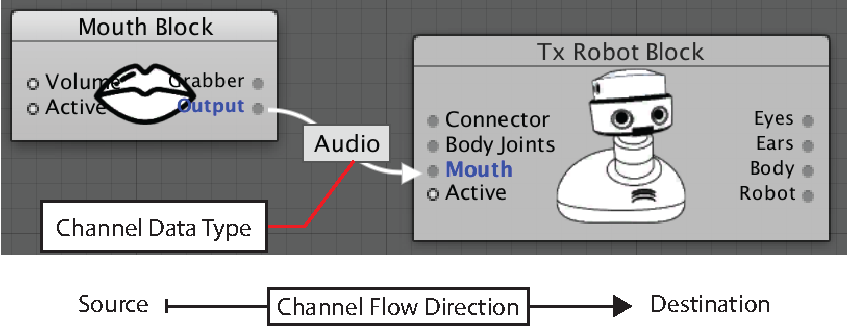
\includegraphics[width=0.8\textwidth]{figures/system/Blocks/Flow.pdf}
\caption{Channel data flow between the blocks.}
  \label{fig:system-blocks-flow}
\end{figure}


\section{Meta-Modeling: Blocks Implementation}

As was described in the design chapter, EDD consists mainly of three set of blocks that can be used to define the body schema transfer model. The design considerations were reflected in the implementation following the same categories for creating meta-blocks. This section describes the details of each block category with the underlying details of the mechanism used in the inter-state of the blocks. 

In order to organize the accessibility to the blocks, each block should define a path in form of ``[Category Name]/[Sub-path]/[Block Name]''. This path is set when the block is implemented in the script. \Listing{lst:blockcode} provides a sample template to declare new meta-blocks. The block class require an attribute of type [ModelBlock] in order to automatically register the block into the graph using the path specified in its argument. Two optional arguments can be added for the icon image and width of the block in pixels in the editor.

\begin{lstlisting}[caption=a definition template class for meta-blocks objects, label=lst:blockcode]
//mandatory attribute, declare this object as being a block in the editor using the specified path, and set an icon image with width of 100px
[ModelBlock("Transfer/Modifier/Block Sample","Icon",100)] 
//the block should be derived from BlockBase class
public class BlockSample : BlockBase 
{
    //internal state variables
    //.....
    //Declare an input channel with data type of XDataType
	[Inlet]
	public XDataType Input{
		set {
		//set internal variables
		}
	}
	//internal block data used for output channel
	YData _outputData;
	//declare an output channel. 
	[SerializeField, Outlet]YEvent OutputY; 
	void Start () {
	    // Initialize block state
	}
	// UpdateState is periodically
	void UpdateState () {
	    //process the internal state of the block
	    //.....
	    //signal outputs
	    OutputY.Invoke(_outputData);
	}
}
\end{lstlisting}


\subsection{Perceptual Blocks Category-set}

This category of blocks are mainly concerned with the user side. The blocks provides a representation of the operator body's state and posture by using \textbf{body state blocks}, which is captured using \textbf{body tracking blocks} , as well as providing to the user information and sensory feedback using  \textbf{feedback blocks}.

\subsubsection{Body State Blocks}

\begin{figure}[b!]
\centering
\captionsetup{justification=centering} 
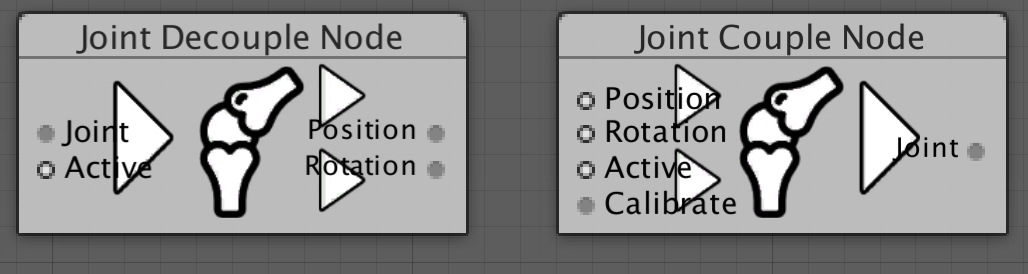
\includegraphics[width=0.8\textwidth]{figures/system/Blocks/Joint.png}
\caption{Joint block, the minimal level of postural schema.}
  \label{fig:system-blocks-joint}
\end{figure}
Body postural representation is designed as a set of blocks that contains the individual joints state. The structure of the blocks follows the previously described Loosely Coupled Modalities (LCM) design pattern in which the structure can be decoupled into smaller regions or grouped back to reconstruct the original region. The minimal region that body structure can be decoupled into is a [Joint] block \Figure{fig:system-blocks-joint}. The joint block contains the spatial attributes represented by a position and rotation channels, which can be captured using [Joint Decouple] block. The position channel accepts a data type of \textit{Vector3} and the rotation accepts \textit{Quaternion} data type. The coordinate system which the joints are represented with is Left-Handed system. Using a singular coordinate system among the spatial blocks is important to decide, so the tracking and representation blocks can use the same system to provide or read the joints data from.

Each joint contains a \textit{Calibrate} input which, when it is triggered, would set the current spatial state of the joint as its initial postural. That is:

\begin{equation}
\begin{split}
Position_{Initial}&=Position\\
Rotation_{Initial}&=Rotation^{-1}\\
\end{split}
\end{equation}
And for each new input value:
\begin{equation}
\begin{split}
Position&=-Position_{Initial}+Position_{Input}\\
Rotation&=Rotation_{Initial}^{-1}\times Rotation_{Input}
\end{split}
\end{equation}

\begin{figure}[b!]
\centering
\captionsetup{justification=centering} 
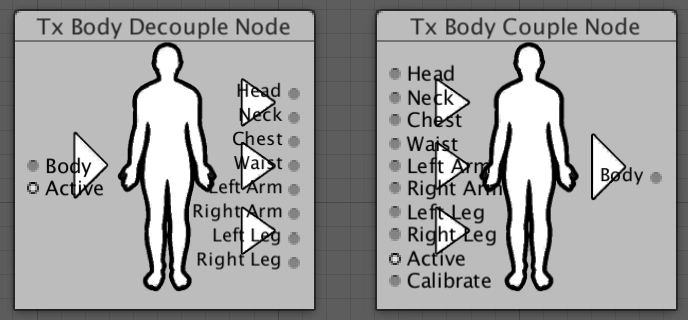
\includegraphics[width=0.8\textwidth]{figures/system/Blocks/Body.png}
\caption{Body decoupling and coupling blocks.}
  \label{fig:system-blocks-body}
\end{figure}

The entire body structure is represented using Body block \Figure{fig:system-blocks-body} which contains a hierarchical structure of the main joints of the spine (waist, chest, neck, and head), two arms and two legs (Left and Right). The body block follows LCM design pattern in which it can supports the decoupling and re-coupling of its sub-structure. Arm block structure is shown in \Figure{fig:system-blocks-arm}. The arm block can be decoupled into four joints (shoulder, clavicle, elbow, and wrist), and a hand. The hand block is structured using five fingers, and each finger has three joints. Finally the leg block is shown in \Figure{fig:system-blocks-leg} and can be decoupled into three joints (hips, knee, and foot). 


\begin{figure}[htpb]
\centering
\captionsetup{justification=centering} 
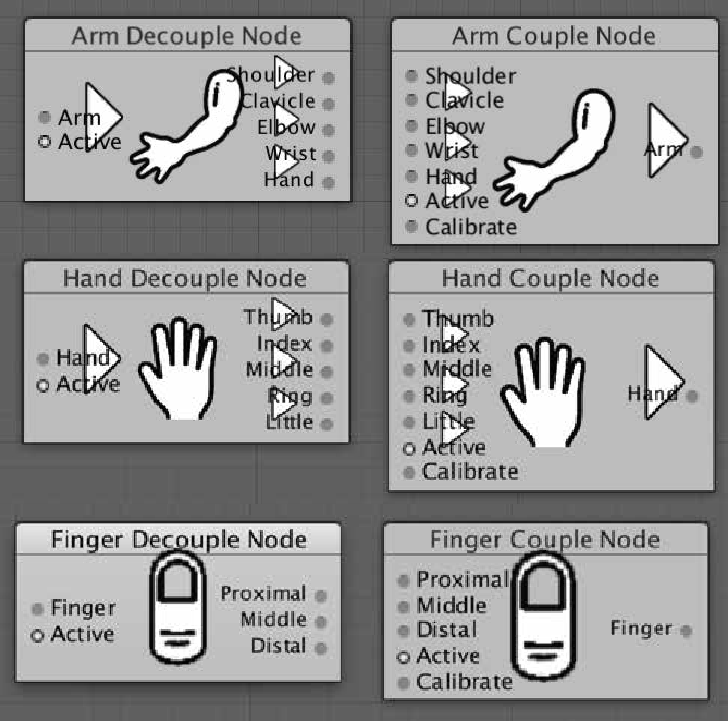
\includegraphics[width=0.8\textwidth]{figures/system/Blocks/Arm.pdf}
\caption{Arm, Hand, and Finger decoupling and coupling blocks.}
  \label{fig:system-blocks-arm}
\end{figure}

\begin{figure}[htpb]
\centering
\captionsetup{justification=centering} 
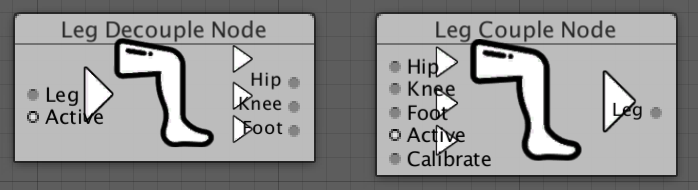
\includegraphics[width=0.8\textwidth]{figures/system/Blocks/Leg.png}
\caption{Leg decoupling and coupling blocks.}
  \label{fig:system-blocks-leg}
\end{figure}

To clarify the benefits of using such highly hierarchical body structure, \Figure{fig:system-bodycoupling} shows an example of how the body parts can be selectively controlled, mapped, and structured. This example shows a single joint controlling two different joints at different levels (head and left arm elbow), while the leg block is mapped into both left and right legs of the body block. Similarly, a single finger block is used to drive three different fingers of the left hand (thumb, index, and little fingers). The data flow type is highlighted on the channels outputs of the blocks. 

\begin{figure}[htpb]
\centering
\captionsetup{justification=centering} 
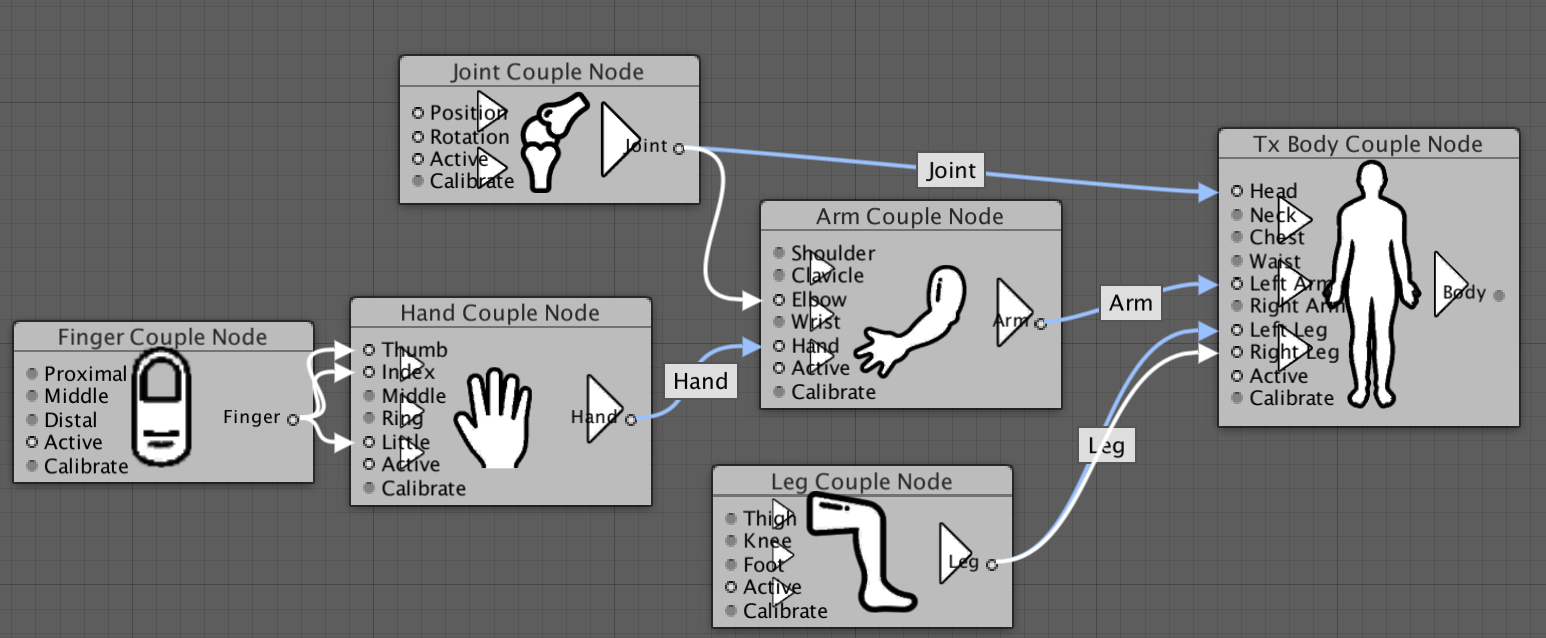
\includegraphics[width=1\textwidth]{figures/system/Blocks/CouplingBody.png}
\caption{An example of Loosely-Coupled Modalities (LCM) to Restructure Postural Schema of the Body.}
  \label{fig:system-bodycoupling}
\end{figure}

\subsubsection{Body Tracking Blocks}
%eyegaze
%body tracking
%hand tracking


For body spatial tracking, various technologies and systems has been tested and integrated into the meta-modeling editor. Each tracking system provides advantages and use cases which varies its functionality from the other systems. \Table{table:system-trackingsystems} summarizes a comparisons between the used systems in term of target body regions required to be tracked (usability), the degree of complexity the system would require to setup and use, and finally the accuracy and robustness of the tracking. Within the tested systems, a trade off between the three criteria was required when deciding the target system to be used in the model. Each of these systems uses different method and procedure for motion capture, and each has its advantages and disadvantages which would constraint the design of the system. In the listed systems, two distinct categories of tracking mechanism are used:


\begin{table}[t!]
\footnotesize
\centerline{
\begin{tabular}{|l|l|l|l|l|l|l|l|}
\hline
\rowcolor[HTML]{EFEFEF} 
\multicolumn{1}{|c|}{\cellcolor[HTML]{EFEFEF}}                                  & \multicolumn{5}{c|}{\cellcolor[HTML]{EFEFEF}Usability} & \cellcolor[HTML]{EFEFEF}                             & \cellcolor[HTML]{EFEFEF}                             \\ \cline{2-6}
\rowcolor[HTML]{C0C0C0} 
\multicolumn{1}{|c|}{\multirow{-2}{*}{\cellcolor[HTML]{EFEFEF}Tracking System}}  & Head   & Hands   & Fingers   & Body   & General   & \multirow{-2}{*}{\cellcolor[HTML]{EFEFEF}Complexity} & \multirow{-2}{*}{\cellcolor[HTML]{EFEFEF}Robustness} \\ \hline
\cellcolor[HTML]{EFEFEF}Oculus HMD                                            & $\surd$    & $\times$    & $\times$      & $\times$        & $\times$      & Low                                                  & High                                                 \\ \hline
\cellcolor[HTML]{EFEFEF}Oculus Touch                                      & $\times$   & $\surd$     & $\triangle$       & $\times$        & $\times$      & Medium$^{1}$                                                  & High                                                 \\ \hline
\cellcolor[HTML]{EFEFEF}Leapmotion                                              & $\times$   & $\surd$     & $\surd$       & $\times$        & $\times$      & Low                                                  & Medium                                               \\ \hline
\cellcolor[HTML]{EFEFEF}5DT Data Glove                                          & $\times$   & $\surd$     & $\surd$       & $\times$        & $\times$      & Low                                                  & High                                                 \\ \hline
\cellcolor[HTML]{EFEFEF}Neuron Perception                                       & $\surd$    & $\surd$     & $\triangle$   & $\surd$         & $\times$      & Medium                                               & Medium                                               \\ \hline
\cellcolor[HTML]{EFEFEF}OptiTrack                                  & $\surd$    & $\surd$     & $\times$      & $\surd$         & $\surd$       & High                                                 & High                                                 \\ \hline
\end{tabular}
}
\begin{tablenotes}
$^{1}$ Oculus Touch require the user to hold them while operation, which is not a seamless tracking method.
\end{tablenotes}
\centering
\captionsetup{justification=centering} 
\caption{A comparison between body tracking systems based on the usability, complexity, and robustness.}
\label{table:system-trackingsystems}
\end{table}


\begin{enumerate}
\item \textbf{Optical tracking}: In this category, the motion capture system uses a single or several cameras (or light sensors) to triangulate the 3D position of a set of points defining the tracked object. Based on this triangulation process, the points are matched with a predefined model representing the tracked object, and then the position and orientation of the object can be calculated. These systems require a calibration process for the cameras to extract the intrinsic parameters (related to the lens of the camera, sensor size, ...etc), and extrinsic parameters (related to the spatial distribution of the cameras when multiple were used, and the location and orientation of the reference ground plane). Since a continuous visibility of the points by the tracking cameras is required, these systems deliver poor tracking when the points were occluded. \\
Two types of tracking systems uses optical tracking:

\begin{itemize}
\item Active type: the tracked points of this system have an illuminating light source (usually within the infrared spectrum) that can be distinguishably tracked from other non relevant points in the environment. Both Oculus HMD and Oculus Touch uses this mechanism for tracking.

\item Passive type: in this type of systems, the tracking cameras are equipped with a special light source (usually infrared light source) that illuminate the environment. The markers or features that needed to be tracked usually reflect the illuminated light back to the camera (usually using a retroreflective material), and thus can be extracted. In this type of systems, usually high noise occur and would require tuning of the environment and the camera parameters. The advantages however is low cost and the flexibility to define custom tracking props. Both Naturalpoint OptiTrack and Leapmotion systems uses passive tracking.
\end{itemize}

\item \textbf{Non-optical type}: In optical tracking category, the motion capture systems required a reference tracking camera and continuous visibility of the tracked features. The non-optical type however, does not require tracking source, thus can perform better in terms of occlusion and freedom in motion. The tracking mechanism however is different for each type of systems. For the used systems, two types of motion tracking is used:

\begin{itemize}
\item Inertial type: systems of this category use intertial motion sensors, or most commonly, inertial measurement units (IMUs) that combines three different sensors: gyroscope, magnetometer, and accelerometer on a miniature device, and uses sensor fusion algorithms to measure the rotational rates of the unit. Since these units use relative motion and accumulate the results of the internal sensors to calculate the current orientation, a small error also accumulates resulting orientation draft. This error is due to the non-perfect accuracy of the sensors. The system would require calibration procedure (system dependent posture, usually T-Pose) whenever draft occurs. Neuron Perception system uses IMUs to measure the orientation of the body. This system can support various layouts for tracking depending on the number of IMUs used and their location on the suit shown in \Figure{fig:system-neuron-overview}: 1) Full body tracking using 11,18,21, or 32 IMUs, 2) Single arm tracking using 3,6,9, or 11 IMUs, or 3) Upper body tracking using 6,11,21, or 25 IMUs. The calibration procedure for this system is shown in \Figure{fig:system-neuron-calibration}. 

\item Mechanical type: these systems uses directly mounted sensors that measure the mechanical motion of human joints. The sensors are located directly at the joint location to measure its bend. The problem with these systems is they are highly constrained due to the mechanical design, and require exact alignment with the joint. 5DT data glove system uses fiber bending sensors for tracking finger motion.

\end{itemize}
\end{enumerate}



\begin{figure}[t!]
\centering
\captionsetup{justification=centering} 
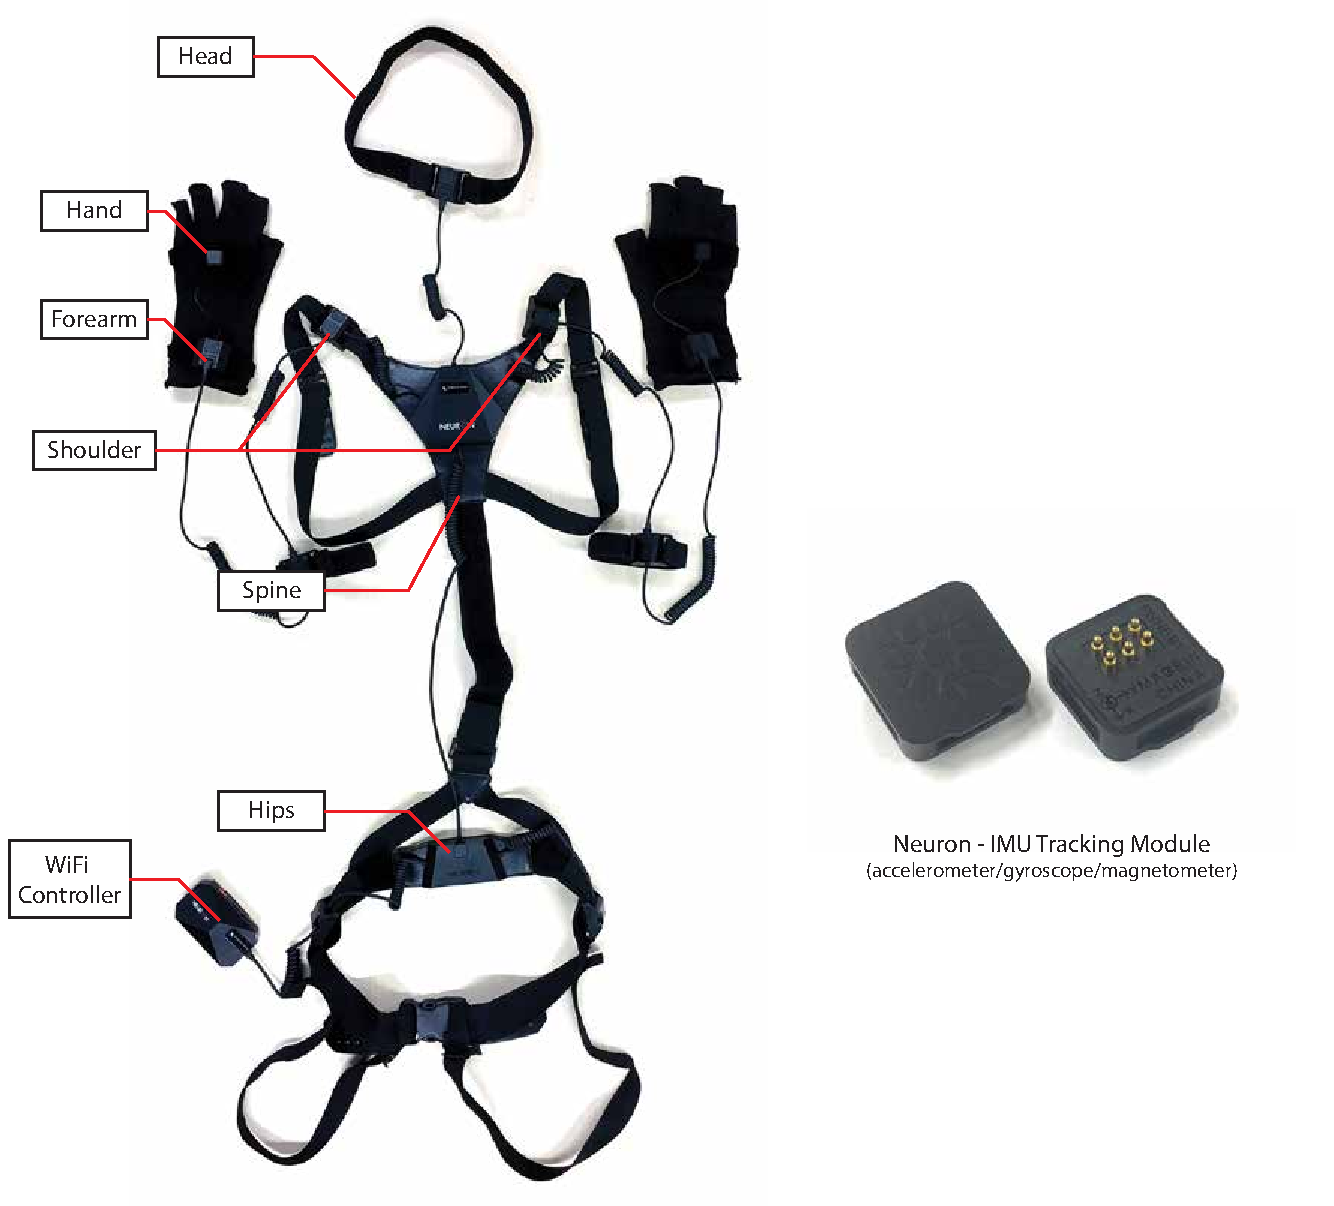
\includegraphics[width=0.8\textwidth]{figures/system/NeuronPerceptron.pdf}
\caption{Full body tracking system (Neuron Perception).}
  \label{fig:system-neuron-overview}
\end{figure}

\begin{figure}[t!]
\centering
\captionsetup{justification=centering} 
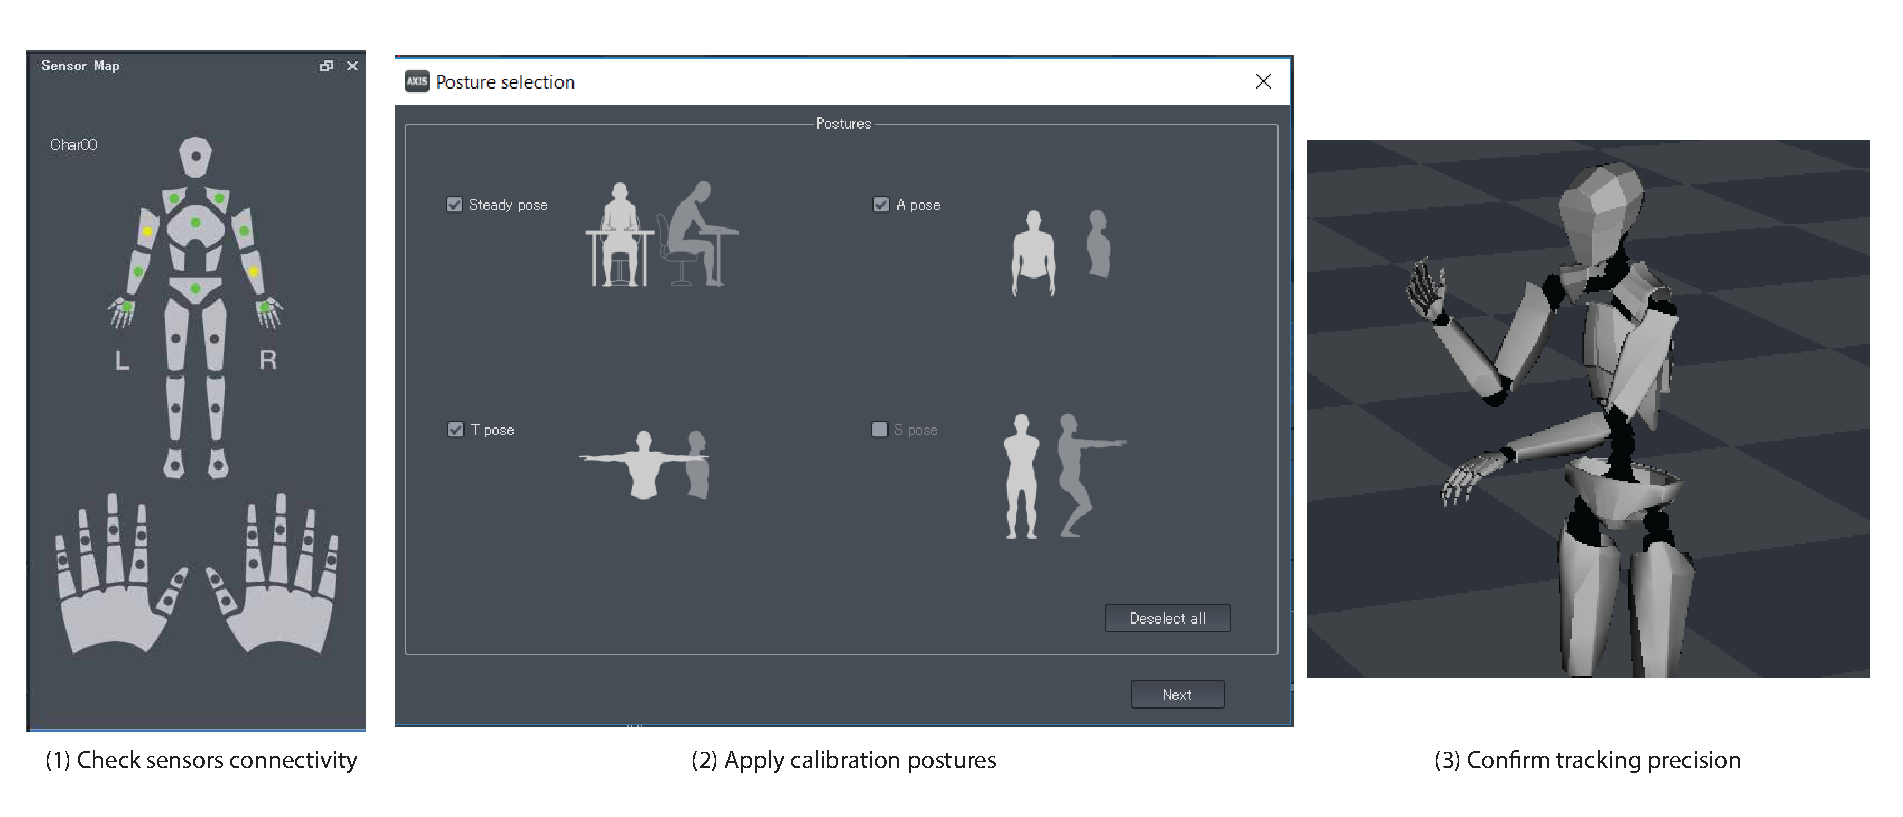
\includegraphics[width=1\textwidth]{figures/system/NeuronCalibration.pdf}
\caption{Calibration process for Neuron Perception system.}
  \label{fig:system-neuron-calibration}
\end{figure}



A combination of multiple systems is also possible in order to acquire the highest robustness with minimum complexity while maintaining the number of joints tracked. For example, to use Oculus HMD to track the head motion while providing the visual and auditory feedback to the user combined with 5DT data glove to track fingers posture, and overall body tracking using Neuron Perception system. 

As part of body state quantification modeling, eye gaze modality provides important information about the area of interest the user is looking at. This modality can be used as supportive input for multi-modal interaction as will be described later in operation and model alteration meta-models. An pupil tracking system was used by embedding dual cameras into the head mounted display. The system uses infrared cameras located behind the lenses of the HMD, and a half mirror placed at $45\deg$. Five infrared LED emitters are embedded into the lens which illuminate the eye pupil. The camera captures the reflected light of the eye via the half mirror. An illustration of the system is shown in \Figure{fig:system-pupillabs-overview}. A custom plugin for Unity3D was developed and integrated which communicates with the camera software. The plugin carries on the calibration procedure which is required per-user before start using the trackers. A 9-points eye fixation calibration is integrated, which maps the captured pupil locations with pre-defined points in 2D space. 120 samples per point (which is about 2 seconds per eye for 60 FPS tracking, in total 18 seconds for all points ) provided good balance between calibration time and accuracy of tracking.

The last modality for capturing user's state is the speech modality. The audio from user side is captured from an attached audio input interface. Although in most cases only a single audio input interface is needed to capture the state of user's speech, however the model supports the use of multiple audio interfaces. For example, in multiple audio input case, its possible to triangulate the position of the audio source using the volume. These types of use cases are application dependant.


\begin{figure}[t!]
\centering
\captionsetup{justification=centering} 
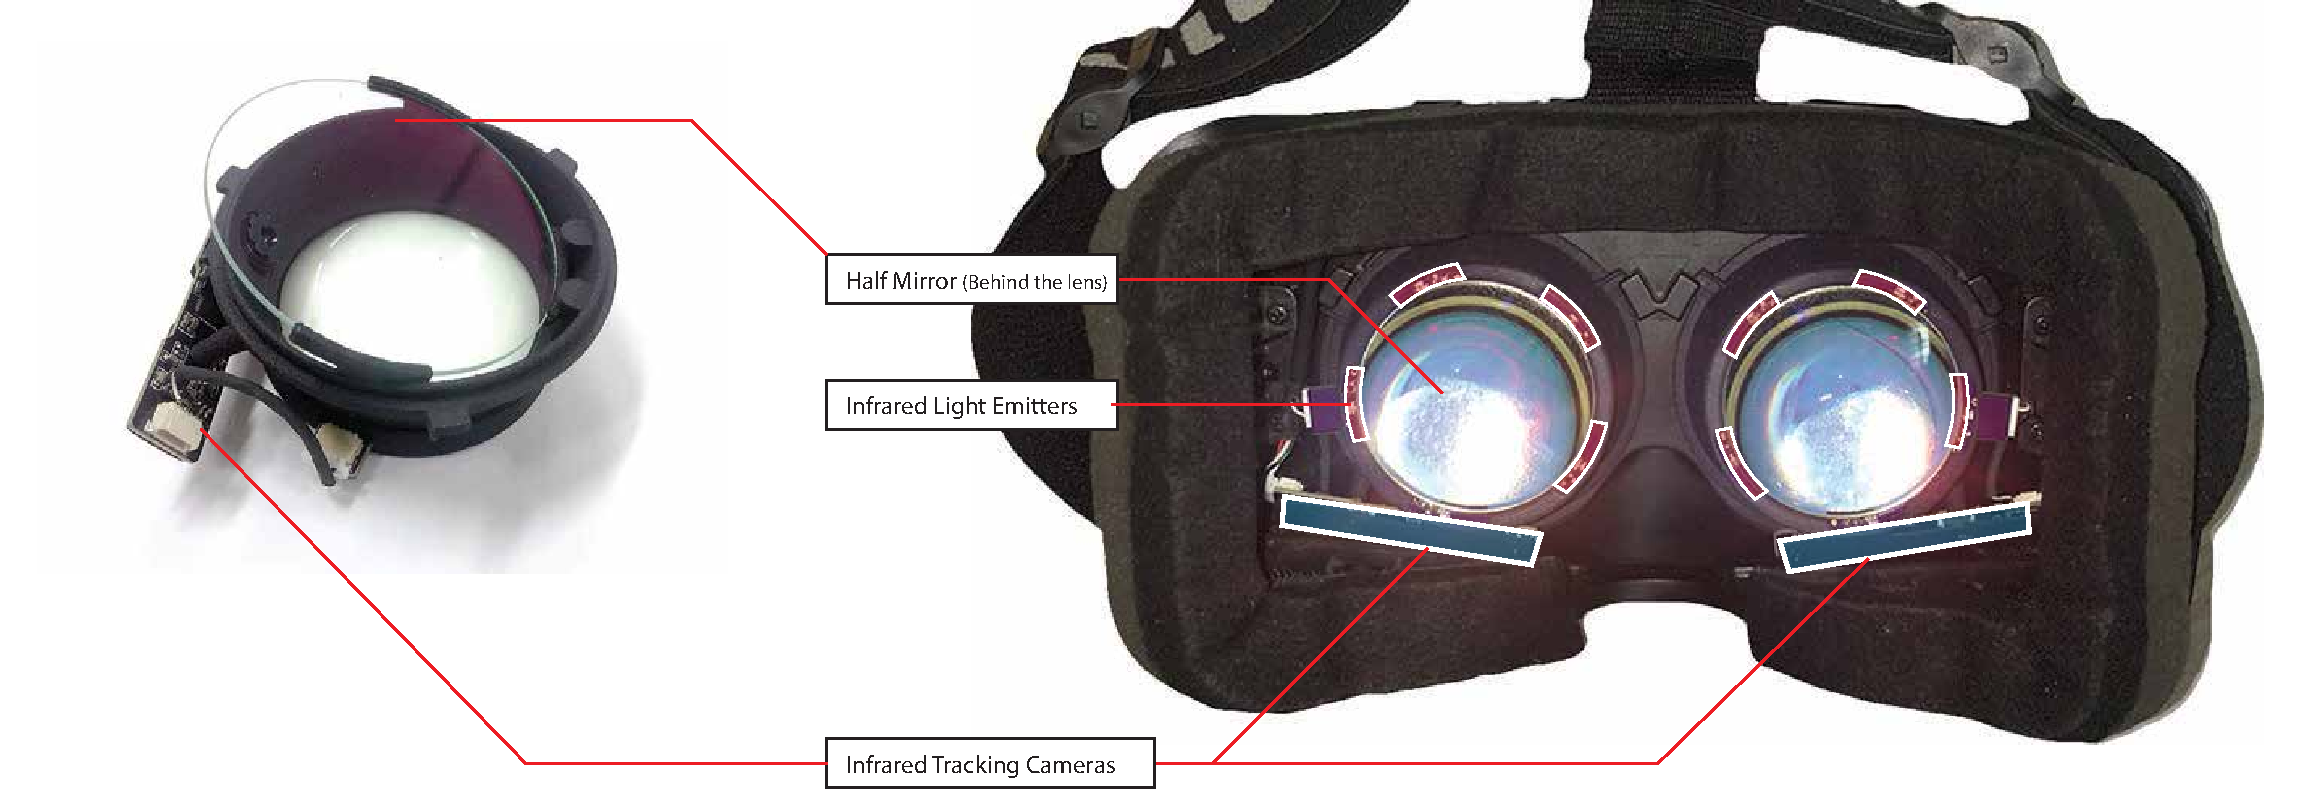
\includegraphics[width=1\textwidth]{figures/system/PupilTracker.pdf}
\caption{Eye tracking module used (PupilLabs + Oculus DK2).}
  \label{fig:system-pupillabs-overview}
\end{figure}




To use in the meta-modeling editor, the tracking systems were encapsulated and integrated as meta-blocks shown in \Figure{fig:system-trackers-blocks}:
\begin{itemize}
\item OptiTrack Block: Communicates with an optiTrack server that runs the tracking system. The node requires to specify the target server IP address. For each block, the name of the target tracked object should be specified in its block parameters. When the meta-model runs, the object data is output as [Joint] data channel.

\item HMD Block: Handles the tracking of the connected HMD. The block provides two outputs: [Joint] for the spatial position and orientation of the HMD, and [Mounted] as a boolean channel indicating whether the HMD is being used or not (compatible with Oculus CV1/HTC Vive HMDs).

\item Neuron Block: Similar to OptiTrack Block, it also requires to specify the server IP address running Neuron Perception service. This node requires to specify the ActorID when more than one tracking suit is being connected. The block outputs [Body] data structure containing the entire tracked body joints data.

\item Leapmotion Block: Provides accessibility functions to leapmotion tracking. Requires to specify the target hand to track (Left or Right), and it outputs [Hand] data. [Fist] provides whether the hand is closed or not as floating point value.

\item 5DT Data Glove Block: Similar to Leapmotion, requires to specify the target hand to track, and it outputs fingers information on the [Hand] output channel.


\begin{figure}[t!]
\centering
\captionsetup{justification=centering} 
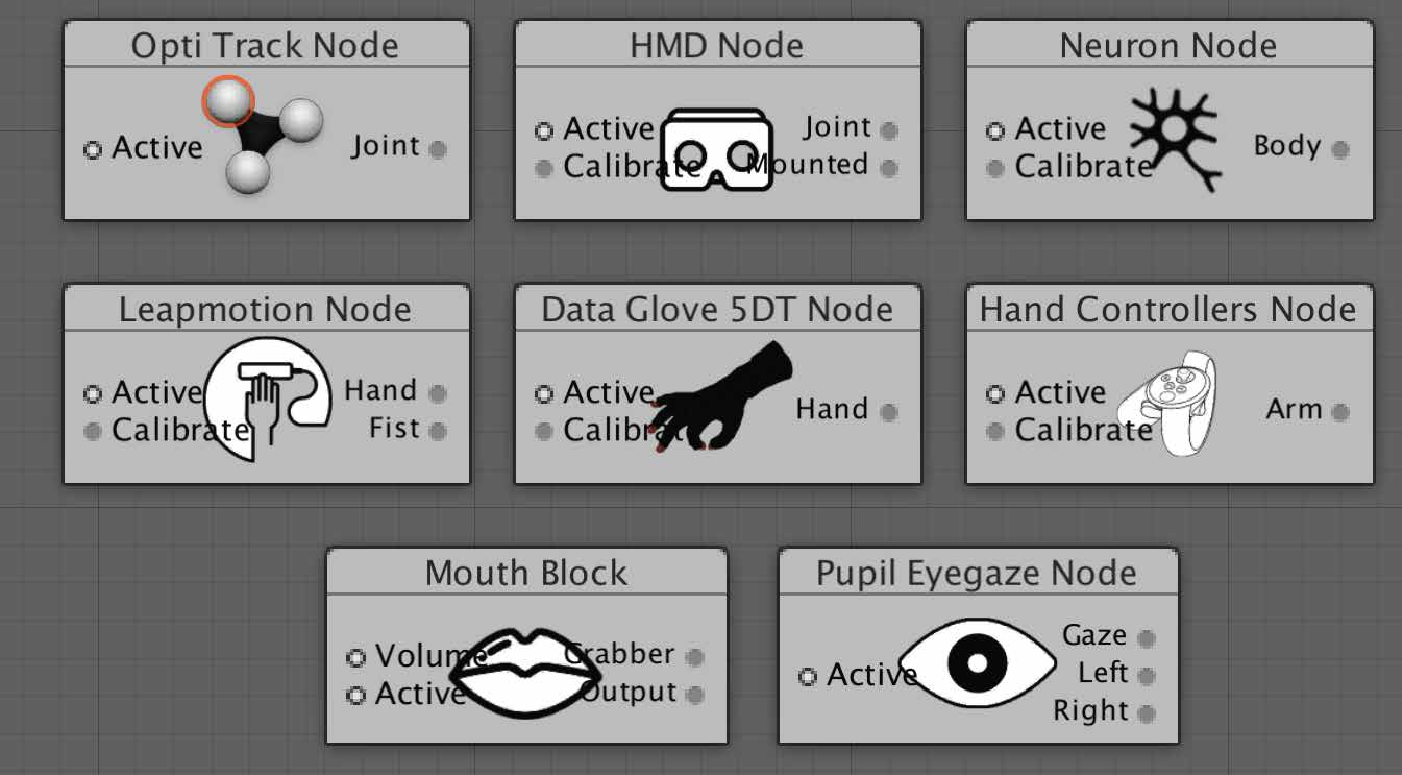
\includegraphics[width=1\textwidth]{figures/system/Blocks/Trackers.pdf}
\caption{Body state tracking blocks.}
  \label{fig:system-trackers-blocks}
\end{figure}

\item Hand Controllers Block: Uses Oculus Touch to track hands position and fingers bending. Outputs [Arm] structure containing the estimated position of the hand relatively to the HMD position.

\item Mouth Block: Connects to an audio input interface, and provides the sampled audio on [Output] channel. It is possible to indicate the sampling rate in its settings, default set to 16,000Hz.

\item Pupil Eyegaze Block: Uses the functionality of Pupillabs eye tracking hardware to measure the pupil gaze position. Outputs both [Left] and [Right] values for both eyes, and the estimated looking position on [Gaze] channel. Data used is a 2D value vector [Vector2].

\end{itemize}




\subsubsection{Feedback Blocks}
%ears 
%mouth


Feedback blocks mainly communicates the meta-model perceptual states back into the user. Within the current scope of this thesis, three different types of feedback modalities are explored and integrated into the EDD framework and meta-modeling editor:


\begin{figure}[b]
\centering
\captionsetup{justification=centering} 
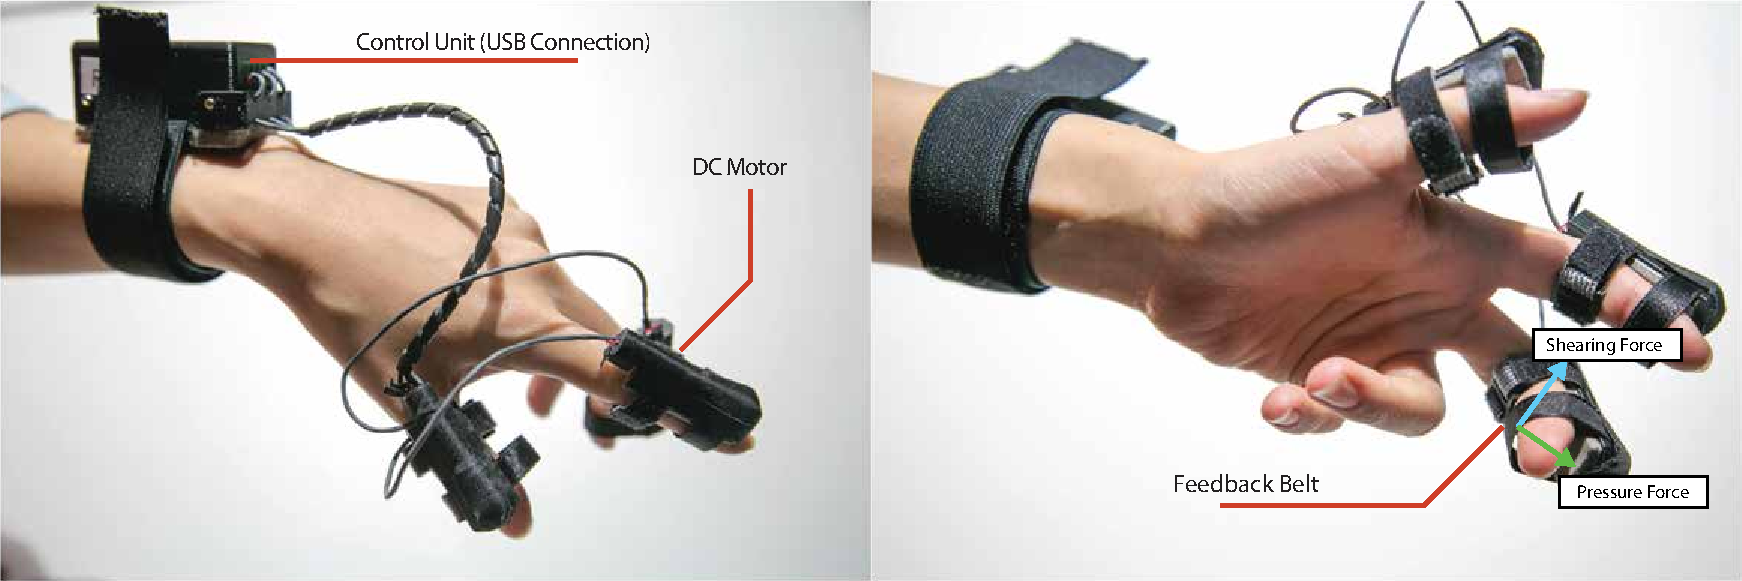
\includegraphics[width=1\textwidth]{figures/system/GGDisplay.pdf}
\caption{Fingers force feedback display.}
  \label{fig:system-GGDisplay}
\end{figure}

$\bullet$ Visual Feedback: transforms stereo images input into a displayable format to be presented into the user's vision. The visuals are directed into [Vision] data type which contains dual textures of type Texture2D. These images are either captured from representation blocks, or are generated from transfer blocks. Depending on the display device used (HMD, Monitor, ...etc), parameters related to the field of view and aspect ratio of the device should be specified. In the meta-blocks, these functionalists are encapsulated and are automatically calculated, however it is still possible for the designer to alter these settings.

$\bullet$  Auditory Feedback: plays back audio samples stream into an output audio interface at the user's side, and represented as [Ears] module. Samples are encapsulated into an [Audio] data type that can handle multiple audio channels, and different sampling rates. For audio playback, the sampling rate by default is set to 48,000Hz, but can be changed by the designer.

$\bullet$ Haptic Feedback: communicates with a haptic interface connected to the user's side, and can provide both force and tactile feedback information into the device. Both data are represented using [Haptic] data structure. Force feedback is a three-directional vector3 which provides the 2D (X, Z) tangential force along the surface of the display, and the perpendicular (Y) pressure force on the display surface. Currently, Gravity Grabber \cite{minamizawa2007gravity} type of displays are supported for force feedback. A custom display has been developed which can provide horizontal (X) shearing forces, and the perpendicular (Y) pressure forces for three fingers of each hand \Figure{fig:system-GGDisplay}. For tactile feedback, the data is stored as an array of floating points within the range of [-1,1] representing the signal captured by a vibrotactile sensor, or generated in software using a transfer block. The sampling rate for this signal is less than 2000Hz samples (representing a maximum frequency of 1000Hz which is the limit of Pacinian corpuscle receptors in the skin). To display the tactile data, a vibrotactile actuator can be used by directly connecting it to an output audio interface and specify the interface ID in the settings of the haptic block.

\begin{figure}[htbp]
\centering
  \captionsetup{justification=centering}
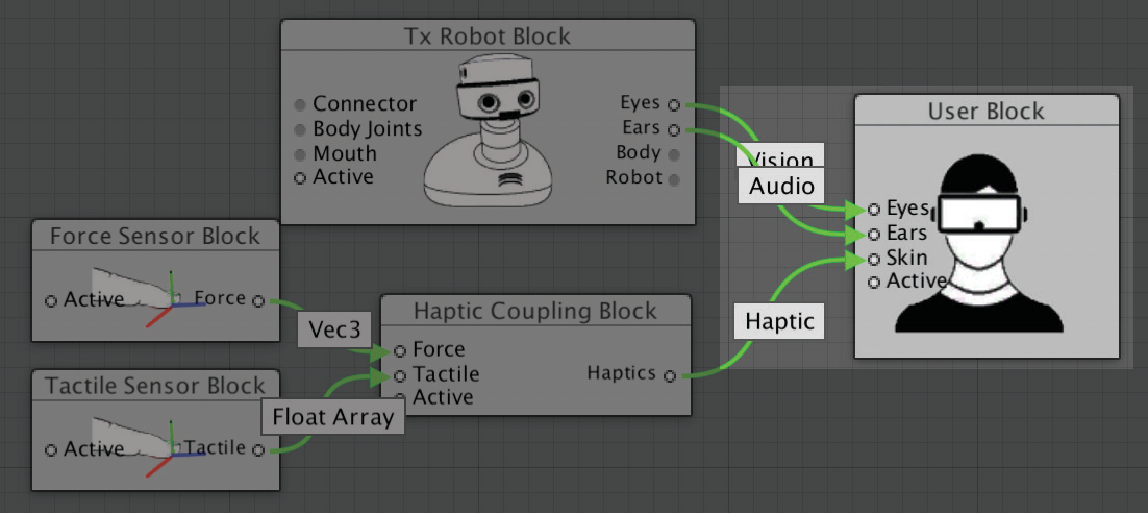
\includegraphics[width=0.8\textwidth]{figures/system/Blocks/UserBlock.pdf}
\caption{User feedback block meta-model example.}
  \label{fig:system-userblock}
\end{figure}

Since all these modalities are related to the user feedback, a single [User] block \Figure{fig:system-userblock} that provides the functionality to receive the various perceptual input has been designed and integrated into the meta-modeling editor. The block receives three inputs representing the Eyes, Ears, and Skin modalities that corresponds to the visual, auditory, and haptic feedback respectively.



\subsection{Representation Blocks}

This set of meta-blocks communicates with the used body representation. It facilitates the process of transferring the information flow between the meta-model and the representation type used. Two main types of representations are used in this thesis: physical and virtual type. The physical type communicates with a robotic form located at the user side as a peripheral device, or remotely connected over the network, and controls its physical state such as servo link driving or captures sensory information from it, such as tactile sensors. And the virtual type mainly communicates with Unity3D editor into a virtual character (humanoid or non-humanoid) to control its body postural. Generally speaking, representation model blocks are considered as mirroring the functionality of perceptual model, that is the for each input of representation blocks a corresponding output from perceptual blocks and vice versa.

The first block type for the body model is the postural blocks. The control mechanism for the postural of the representation is driven by the [Body] data type that defines the new body schema from the user. Different approaches for control is dependant on the \textit{Representation Engineer} choice. For example, the driving can be done using Forward Kinematics (FK) model (direct drive) in which the joints angle is directly applied from the input body joints data. For example, 3 DoF telexistence robot uses forward kinematics to drive the head motion of the robot from the head joint of the body. A 6 DoF robot (with parallax motion type) would use a different approach to calculate robot's joints angle from head position, using Inverse Kinematics (IK) model to drive the parallax joints from head position and rotation. The postural blocks should provide compatible data channel to the representation used, for example a network-based communication is used, a combination of UDP and TCP protocols can be used to bridge the data flow from Unity3D to the robot side, and for peripherals connected directly to the user side pc, a serial communication protocol can be used to deliver the control signals to the used peripheral. The EDD framework provides an abstraction to the communication protocol used, so the same block can be reused for different representations. The  \textit{Representation Engineer} can either develop new protocols to communicate with the hardware used, or to build on to of the exciting protocols used in the framework. The physical toolkit in \Section{impl:toolkit} provides building blocks for developing the representation hardware while maintaining the support to EDD framework representation blocks. The toolkit discussed also includes important details about media streaming optimization for various types of sensory modalities, mainly for the real-time visual feedback. 

\begin{figure}[htpb]
\centering
  \captionsetup{justification=centering}
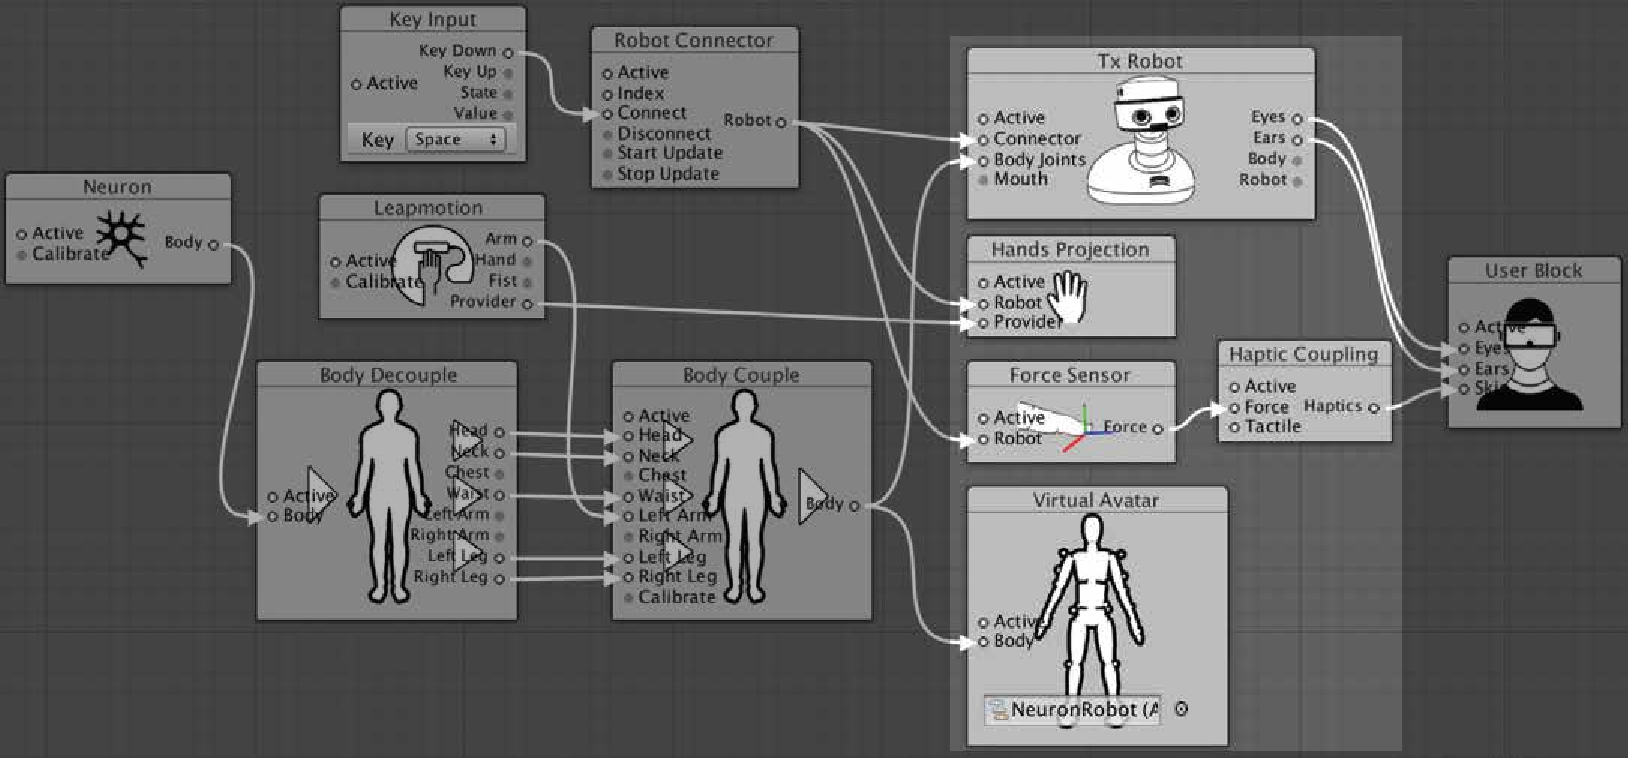
\includegraphics[width=1\textwidth]{figures/system/Blocks/Representation.pdf}
\caption{Using multiple blocks types for representation.}
  \label{fig:system-representatio-blocks}
\end{figure}


The other block type for the representation blocks is the sensory blocks. These blocks are responsible to deliver various modalities information back to the meta-modeling editor. \Figure{fig:system-representatio-blocks} shows an example of using both postural and sensory representation blocks used in parallel for two different types of bodies. [TxRobot] block encapsulates the postural modality function, and provides the sensory feedback on its outputs. The [Force Sensor] is used as a separate module since the number of sensors can vary based on the application. [Hands Projection] block provide the functionality for representation alteration meta-modeling in which it streams the virtual representation of the hands into the robot side. Finally, [Virtual Avatar] block communicates with Unity3D character model to control its postural state based on the shared [Body] input. In this example, both representations are driven by the same body input.



\subsection{Transfer Blocks}

The final category of meta-blocks is the Transfer type. This category contains a wide variety of functions and modifiers which can be general purpose type (e.g. mathematics, image processing, body mapping alteration, ...etc) to a very application specific blocks (e.g. layered perception, motion transformation, ...etc). 

\begin{figure}[htpb]
\centering
  \captionsetup{justification=centering}
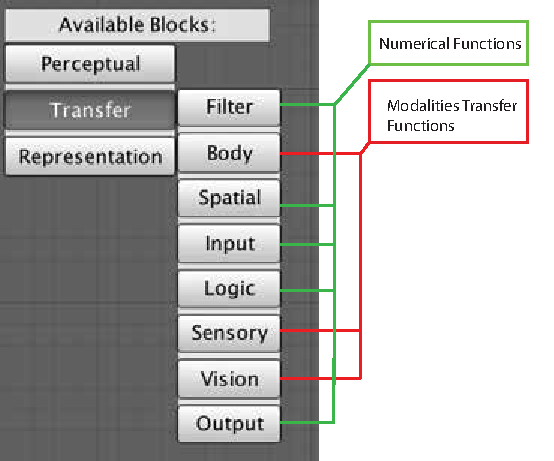
\includegraphics[width=0.8\textwidth]{figures/system/Blocks/TransferBlocks.pdf}
\caption{List of transfer blocks sub categories.}
  \label{fig:system-transfer-blocks}
\end{figure}

The transfer blocks are used as a middle function to modulate the data flow between the representation and user blocks. Also it can be used to apply logic operations on perception, for example activate or disable certain modalities channels flow based on behaviours or body state. A list of transfer blocks categories is shown in \Figure{fig:system-transfer-blocks}.


\begin{figure}[t!]
\centering
  \captionsetup{justification=centering}
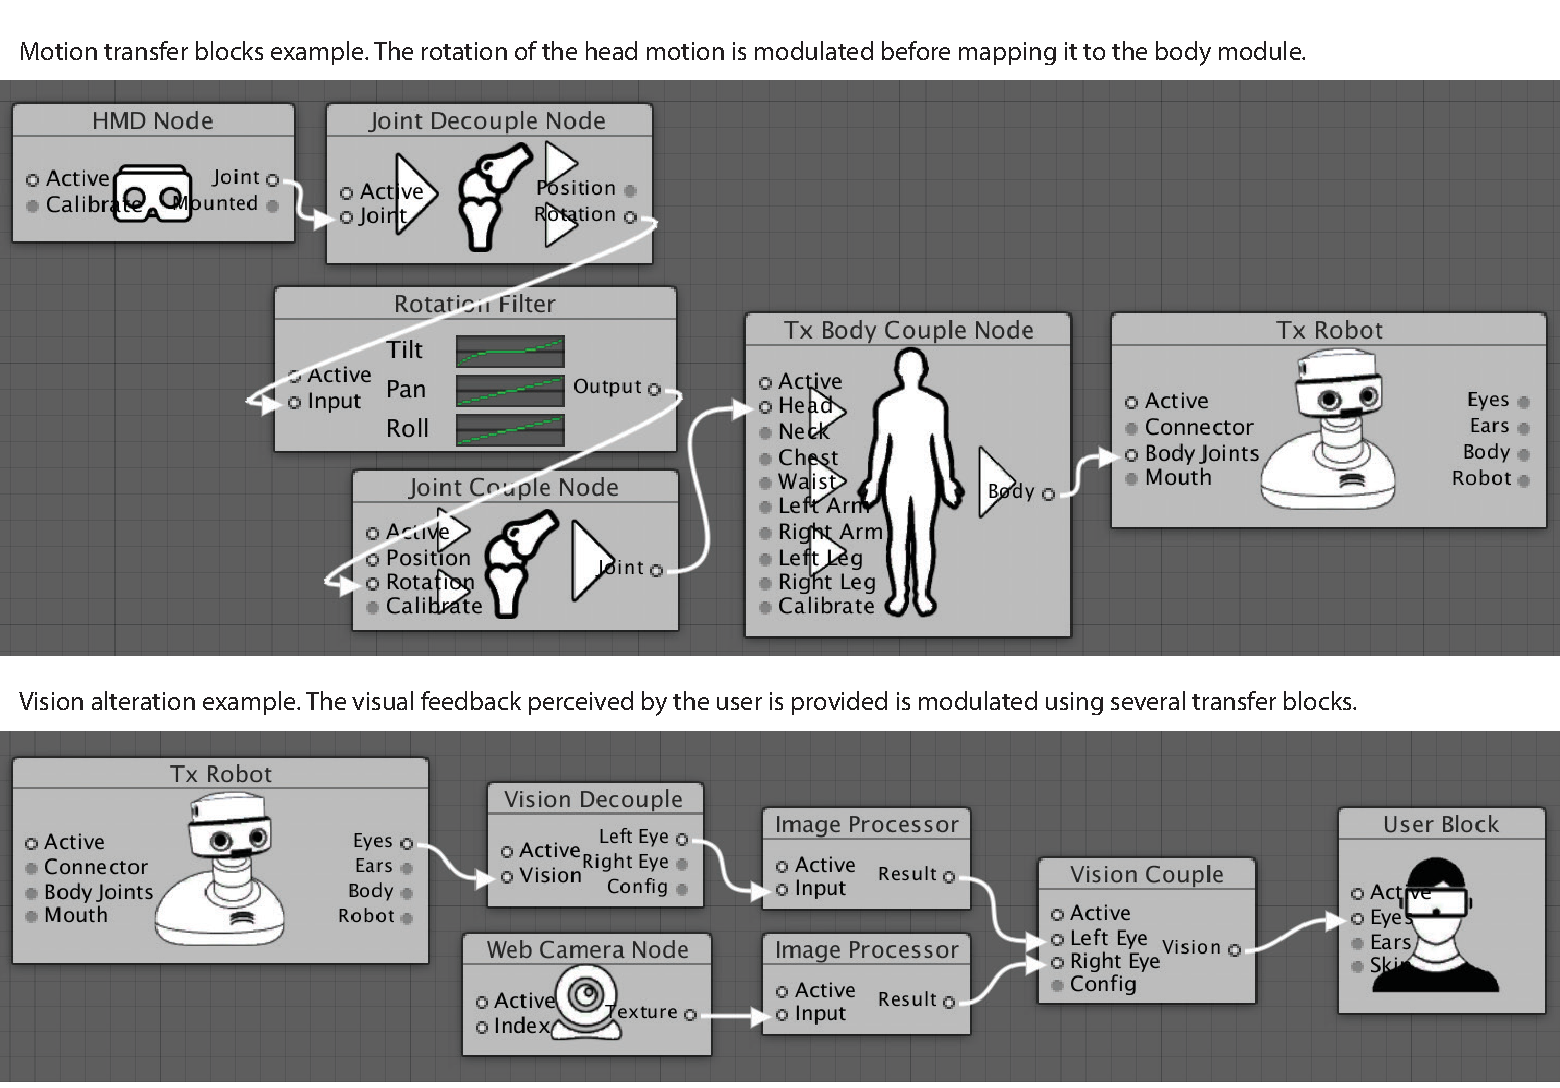
\includegraphics[width=1\textwidth]{figures/system/Blocks/TransferExample.pdf}
\caption{Examples of using transfer blocks to modulate body and visual modalities.}
  \label{fig:system-transfer-example}
\end{figure}

Examples of using transfer blocks to modulate body mapping and perception feedback are shown in \Figure{fig:system-transfer-example}. The first example highlights the use of spatial alteration filter block [Rotation Filter] to modulate head joint rotation into a nonlinear mapping. Three different mapping curves can be defined for each rotational axis (Tilt, Pan, Roll), which acts as a function for each angle. The second example shows a higher level of perception editing. In this example, the vision input modality for the user is altered using two different sources. The robot block's vision is decoupled into separate eyes using [Vision Decouple] transfer block, and then is processed using [Image Processor] transfer block. The image processor block uses a program written in shader language (HLSL) which runs inside the block process to produce a new image on its Result output channel. Robot's vision is mapped into the left eye of the user, while the right eye is mapped to a different source using [Web Camera] representation block. 



\section{Physical Toolkit Development}
\label{impl:toolkit}

As a part of realizing the idea of Embodied-Driven Design on a larger scale, a general purpose physical toolkit was developed through several iterations and prototypes along the development of embodiment framework and the meta-modeling editor. The toolkit design considerations were discussed previously in the design chapter in \Section{concept:toolkit}. The implementation process and details of this toolkit is discussed here.

An overview of the different prototypes that has been developed is illustrated in \Figure{fig:system-txkit-iterations}, and the description of each iteration considerations and requirement is shown in \Table{fig:system-txkit-iterations}. Iterations A-B were highly application specific designs and mainly used for representation alteration purpose. Iteration C was a base step for developing higher performance toolkit using better optics and vision system than the previous generations, and has been used as a part of model alteration meta-modeling. And iteration D is the current design which provides a balance between performance and usability. 

Along the hardware development of the robots, a corresponding software architecture was developed to facilitate the usability of the toolkit and to make it compatible with the Embodiment framework. Both the hardware and the software are highly modular and reusable. 

\begin{figure}[htbp]
\centering
\captionsetup{justification=centering} 
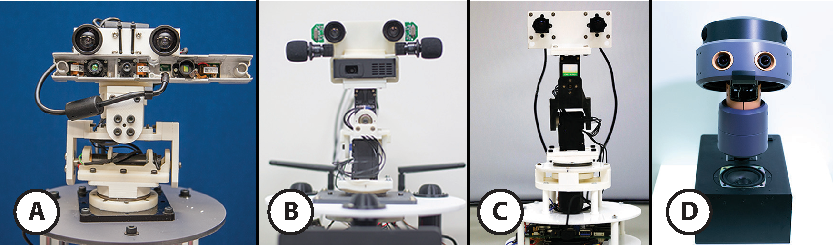
\includegraphics[width=1\textwidth]{figures/system/TxKitIterations.pdf}
\caption{Physical toolkit design iterations. }
  \label{fig:system-txkit-iterations}
\end{figure}


\begin{table}[t!]
\footnotesize
\centerline{
\begin{tabular}{|l|l|l|l|l|}
\hline
\rowcolor[HTML]{C0C0C0} 
\textbf{Iteration}                                                                             & \textbf{A}                                  & \textbf{B}                                       & C                                                           & D$^{*}$                                                           \\ \hline
\cellcolor[HTML]{EFEFEF}\textbf{\begin{tabular}[c]{@{}l@{}}Development \\ Year\end{tabular}}   & 2014                                        & 2015                                             & 2016                                                        & 2017                                                       \\ \hline
\cellcolor[HTML]{EFEFEF}\textbf{Application}                                                   & \multicolumn{2}{c|}{\begin{tabular}[c]{@{}c@{}}Enforced \&\\ Mutual Telexistence\end{tabular}} & \begin{tabular}[c]{@{}l@{}}Layered \\ Presence\end{tabular} & \begin{tabular}[c]{@{}l@{}}General \\ Purpose\end{tabular} \\ \hline
\cellcolor[HTML]{EFEFEF}\textbf{Requirement}                                                   & Depth Sensor                                & Projection Module                                & High performance                                            & Usability                                                  \\ \hline
\cellcolor[HTML]{EFEFEF}\textbf{\begin{tabular}[c]{@{}l@{}}Meta-Model\\ Category\end{tabular}} & \multicolumn{2}{c|}{\begin{tabular}[c]{@{}c@{}}Representation \\ alteration\end{tabular}}     & \begin{tabular}[c]{@{}l@{}}Model\\ alteration\end{tabular} & -                                                          \\ \hline
\end{tabular}
}
%\footnotesize 
\begin{tablenotes}
%\captionsetup{justification=justified,format=plain, font=small} 
\item $^{*}$Developed in a collaboration with Karakuri Products, Inc.
\end{tablenotes}
\centering
\caption{Toolkit design iterations and considerations.}
\label{table:system-toolkit-iter}

\end{table}


%\subsection{Postural Design: Head Motion}
    

\subsection{Hardware Design}

\begin{figure}[htpb]
\centering
  \captionsetup{justification=centering}
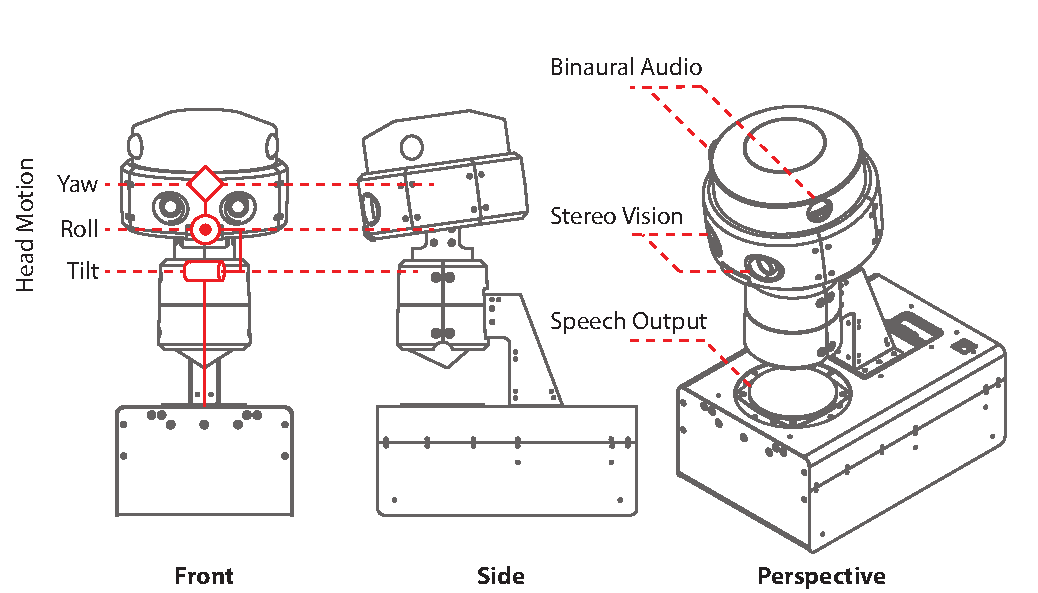
\includegraphics[width=1\textwidth]{figures/system/TxKitDesign.pdf}
\caption{Physical toolkit hardware schematic design.}
  \label{fig:system-txkit-schema}
\end{figure}

The schematic design of the latest toolkit is shown in \Figure{fig:system-txkit-schema}. This design provides the essential modalities for creating general purpose presence experience:
\begin{itemize}
  \setlength\itemsep{0em}
  \item \textbf{Vision:} Stereo camera with fixed interpupillary distance of 65mm (using camera model Ovrvision Pro, or See3CAM CU130 by e-consystems). Each camera has different specifications, but both are suitable for human oriented vision. \Table{table:system-toolkit-cams} provides a list of the important details regarding the selection of the cameras.
  \item \textbf{Auditory:} Binaural microphone set (Audio Technica AT9911). 
  \item \textbf{Communication:} Audio output speaker with an omni-directional design. A custom audio amplifier was added for controlling audio levels. 
  \item \textbf{Body structure:} Motion control using 3 Axis head (Pitch, Yaw, Roll). Servo type motors were used to control rotation position of the robot head motion (Kondo Robots model KRS-4031HV ICS/KRS-4032HV ICS). The mechanical limits for each of the three axes is shown in \Table{table:system-toolkit-motion}.
\end{itemize}





\begin{table}[htpb]
\footnotesize
\begin{tabular}{|l|l|l|}
\hline
                                                   & \cellcolor[HTML]{EFEFEF}\textbf{\begin{tabular}[c]{@{}l@{}}See3Cam\_CU13\\ +H0320KP (S Mount Lens)\end{tabular}} & \cellcolor[HTML]{EFEFEF}\textbf{Ovrvision Pro}                                                          \\ \hline
\cellcolor[HTML]{EFEFEF}\textbf{Count}             & 2                                                                                                                & 1 (stereo camera on board)                                                                              \\ \hline
\cellcolor[HTML]{EFEFEF}\textbf{Image Stitching}   & Software stitch (unsynced)                                                                                       & Hardware stitch (synced)                                                                                \\ \hline
\cellcolor[HTML]{EFEFEF}\textbf{Supported Formats} & \begin{tabular}[c]{@{}l@{}}640x480@60\\ 1280x720@60\\ 1920x1080@30\end{tabular}                                  & \begin{tabular}[c]{@{}l@{}}640x480@90\\ 960x950@60\\ 1280x800@60\\ 1920x1080@30\end{tabular}            \\ \hline
\cellcolor[HTML]{EFEFEF}\textbf{USB Connections}   & 2 x USB3.0                                                                                                       & 1 x USB 3.0                                                                                             \\ \hline
\cellcolor[HTML]{EFEFEF}\textbf{Field of View}     & 89x67                                                                                                            & 115x105                                                                                                 \\ \hline
\cellcolor[HTML]{EFEFEF}\textbf{Quality}           & \begin{tabular}[c]{@{}l@{}}High quality \\ (Raw image from sensors)\end{tabular}                                 & \begin{tabular}[c]{@{}l@{}}Low$\sim$Medium Quality \\ (compression and optics)\end{tabular} \\ \hline
\end{tabular}
\centering
\caption{A comparison between the used cameras in the toolkit.}
\label{table:system-toolkit-cams}
\end{table}


\begin{table}[htpb]
\begin{tabular}{|
>{\columncolor[HTML]{C0C0C0}}l |l|l|}
\hline
Axis & \cellcolor[HTML]{EFEFEF}Min{[}-180,180{]} & \cellcolor[HTML]{EFEFEF}Max{[}-180,180{]} \\ \hline
Tilt & $-20\deg$                     & $20\deg$                      \\\hline
Yaw  & $-90\deg$                     & $90\deg$                      \\\hline
Roll & $-20\deg$                     & $20\deg$                     \\\hline
\end{tabular}
\centering
\caption{Head rotational mechanical limits.}
\label{table:system-toolkit-motion}
\end{table}

\subsection{Software Architecture}
The LCM design pattern is reflected in the design architecture of the software for the framework. \Figure{fig:system-txkit-software} shows the major components used in the framework design and the implementation of the representation blocks. The software is distributed along two sides: robot side, and user side. In the current implementation, the robot side provides the following five services:

\begin{itemize}
  \setlength\itemsep{0em}
  \item \textbf{TxEyes:} responsible for camera access and streaming, handles image capture, encoding, and sending to the user side. Supports the following camera types: 
  \begin{itemize}
  \setlength\itemsep{0em}
  \item Directshow UVC camera drivers, such as webcams.
  \item Ovrvision Pro camera.
  \item Ricoh Theta omni directional camera.
  \end{itemize}
  Video latency in this system is measured to $180\pm20$ms when streaming dual images of size 640x480 at 60 frames per second on a LAN.
  \item \textbf{TxBody:} communicates with the hardware and servo motors. The following body architectures are supported:
  \begin{itemize}
  \setlength\itemsep{0em}
  \item Three axis head control (Pitch, Yaw, Roll).
  \item Six axis body control, such as Torso type systems, controlled by head position \& rotation six values tuple (X,Y,Z,Pitch, Yaw, Roll).
  \item Drone type systems, driven by speed vector for position \& rotation (Speed X,Y,Z/Rotational speed Theta, Gamma, Alpha).
  \end{itemize}
  \item \textbf{TxEars:} provides access to audio hardware, capture, encode and streaming audio data over network to user side. Number of audio channels can be set, by default 2 audio channels (Left, Right) are configured.
  \item \textbf{TxMouth:} handles audio stream input from user side, and responsible for audio playback on the robot side.
  \item \textbf{TxHands:} responsible of displaying operator's body images from an egocentric point of view. Compatible with projector modules.
\end{itemize}



\begin{figure}[t!]
\centering
  \captionsetup{justification=centering}
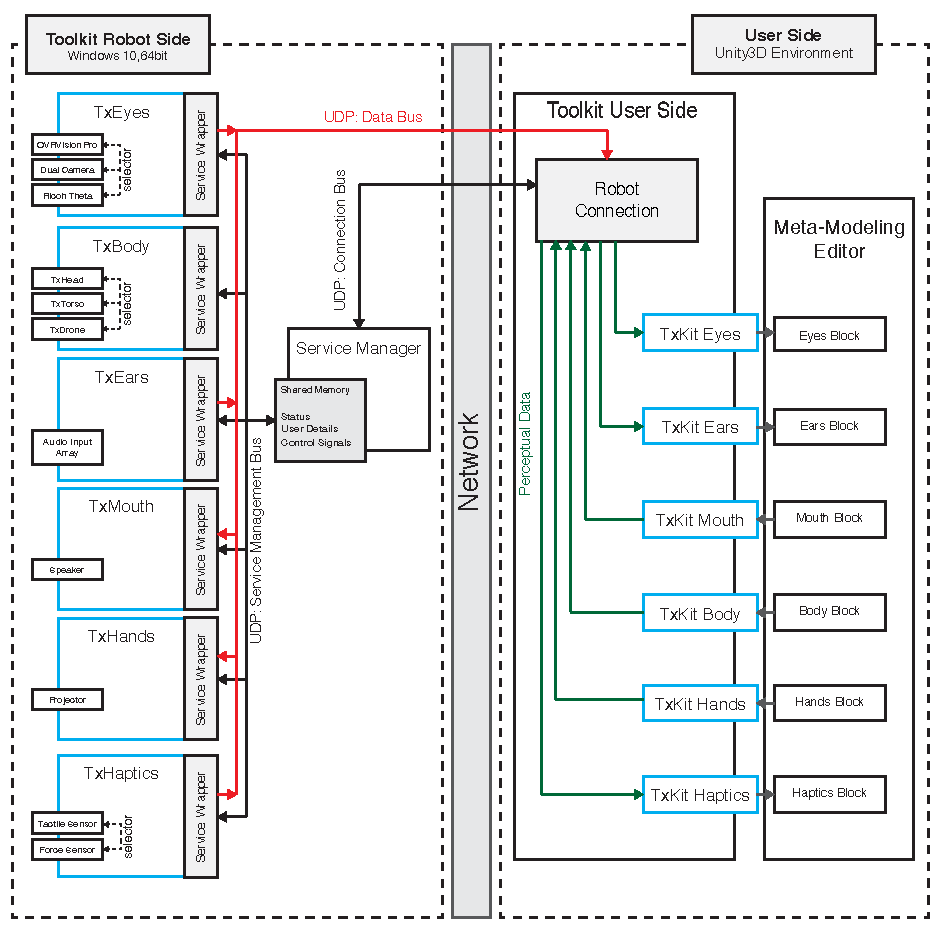
\includegraphics[width=1\textwidth]{figures/system/TxKitSystem.pdf}
\caption{Toolkit software architecture.}
  \label{fig:system-txkit-software}
\end{figure}

Each of these modules is encapsulated as a service, and runs on a separate process in the system, and communicates with a service manager that hosts them over UDP protocol. \Figure{fig:system-txkit-services} shows four different types of services running on the robot side. Each service provides information of their state, as well as the overall resources being consumed by the service (CPU, virtual \& physical memory consumption). A shared memory is used between the processes to provide direct and quick access to the status of the system, user's address, and other control messages. This design provides maximum stability over the system runtime, and reduces the chances of process crashes. Also, as mentioned before, these modules (or services) can run individually depending on the design requirements. For media streaming, encoding, and decoding, GStreamer library was used \footnote{https://gstreamer.freedesktop.org/}. GStreamer is an open source multimedia library which encapsulates the core functions for general video and audio encoders/decoders. In the robot side, H.264 codec was used for video encoding, and Opus codec for audio encoding. Both encoders proved to be the most efficient encoders in term of low latency performance.


\begin{figure}[htpb]
\centering
  \captionsetup{justification=centering}
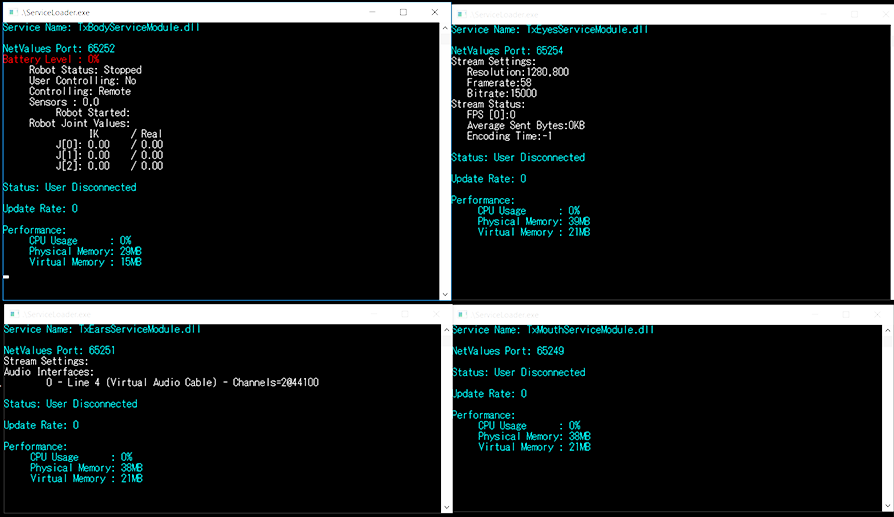
\includegraphics[width=1\textwidth]{figures/system/Services.png}
\caption{Service modules operating on toolkit side.}
  \label{fig:system-txkit-services}
\end{figure}

On the user side, modules are defined to handle the actual communication with the representation. Each of these modules corresponds to a representational block (Eyes, Ears, Mouth, ...etc). The software on the user side is implemented for Unity3D Editor integration under Windows operating system, as this game engine is considered as one of the most user friendly environments for virtual reality related application design.





\subsection{Video Streaming Evaluation}
For achieving close real-time perception streaming over the network, and to minimize the overall latency from the robot side to the user side, an optimized media tool-set were developed and used in toolkit. In the conducted tests, visual latency and image quality were the major considerations in the system design, which they affected the overall experience in robot operation. 

In order to evaluate the streaming performance, a custom measurement software has been developed which calculates the capture-to-display latency of the cameras. The latency measurement system is shown in \Figure{fig:system-txkit-latencymeasure}. To use this system, both the robot side containing the camera to be tested, and the user side should be located physically together. The system uses a display located at the user side that outputs a series of black/white frames which the camera of the streaming side captures. When a frame is displayed, the system records the current time stamp in milliseconds and waits before generating the next frame. The camera side captures, encodes the images into a compressed format such as H264 encoding, and streams the encoded images as a RTP data into the user side over the network medium using UDP protocol. The measurment side receives the RTP stream, decode it and compare the decoded image color value with the currently displayed frame. The system measures the cycle time (or latency time) by calculating the difference between the current timestamp and the displayed frame timestamp. 
 

\begin{figure}[htpb]
\centering
  \captionsetup{justification=centering}
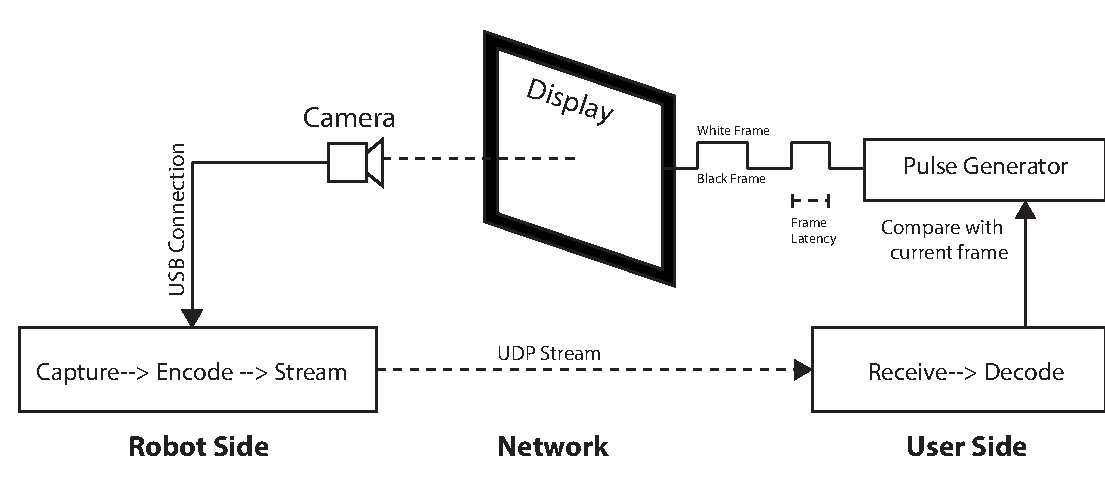
\includegraphics[width=1\textwidth]{figures/system/LatencyMeasurment.pdf}
\caption{Camera capture-to-display latency measurement system.}
  \label{fig:system-txkit-latencymeasure}
\end{figure}

 
The camera module (Model no. See3CAM CU130 by e-consystems) used in the design of the third iteration has been evaluated for streaming performance over the network using the three different quality presets. \Table{table:camera-modes} shows the measured latency for each mode. 


\begin{table}[htpb]
\footnotesize
\begin{tabular}{|l|l|l|l|}
\hline
\rowcolor[HTML]{EFEFEF} 
{\color[HTML]{000000} \textbf{Quality}} & {\color[HTML]{000000} \textbf{\begin{tabular}[c]{@{}l@{}}Resolution\end{tabular}}} & {\color[HTML]{000000} \textbf{Framerate}} & {\color[HTML]{000000} \textbf{Latency (ms)}} 
\\ \hline
\textbf{Low Quality} & 640 x 480 & 60 &  $64\pm8$                                     
\\ \hline
\textbf{Medium Quality} & 1280 x 720 & 60 & $71\pm8$                                           
\\ \hline
\textbf{High Quality} & 1920 x 1080  & 30 &  $95\pm16$                                           
\\ \hline
\end{tabular}
\centering
\caption{Camera streaming quality modes and corresponding latency.}
\label{table:camera-modes}
\end{table}

\section{Vision Bandwidth Optimization}

In the previous section, the evaluation of the vision system showed an acceptable latency measurements (that is less than 100ms), however the effective spatial resolution of the encoded images is relatively low when high frame rate and low bandwidth were required. In this section, an optimization approach is proposed based on the human vision cues which would reduce the bandwidth and performance requirements significantly.

\subsection{Problem with current streaming systems}

Recent advances in virtual reality display systems began to offer end users immersive and high fidelity experiences in a rather accelerating manner. Current Head Mounted Displays (HMD) such as Oculus, Vive, and Samsung GearVR offer wide field of view (FoV) displays ($100\deg\sim120\deg$) with a pixel density of $100\sim175$ per degree at refresh rate ranging from $60\sim90$ frame per second (FPS). In future, expected HMDs are to offer much higher resolution and refresh rate than now in order to enhance the visual experience and immersion towards human eye. However, such visual experiences would require high processing bandwidth to deliver such information stream to the HMD, and performance would decrease exponentially based on the target pixel density and linearly based on the target frame rate. 

On one hand, virtual reality applications that run locally would only require a system capable to operate at such high bandwidth, which is mostly addressed by hardware manufacturers. On the other, Telexistence and Telepresence systems would suffer more at addressing this problem due to network bandwidth limitations. Even with the current standard compression codecs such as MJPEG, H264/MPEG-4, and VP8 will have limited bitrate to accommodate for network streaming. Also, in this type of systems, encoding/decoding are required before streaming and after receiving the image stream, which performance is also dependent on the pixel resolution of the images. Extending the problem for omnidirectional type cameras which sends the entire $360\deg$ view, the resultant pixel resolution of the equirectangular image (the stitched omnidirectional 2D image) would increase 5 to 8 times more than the limited field of view pinhole cameras image type (at $90-110\deg$). As a consequence, the performance of encoding and streaming would increase the latency and decrease the overall experience for Teleoperation. 


\begin{figure} [t!]
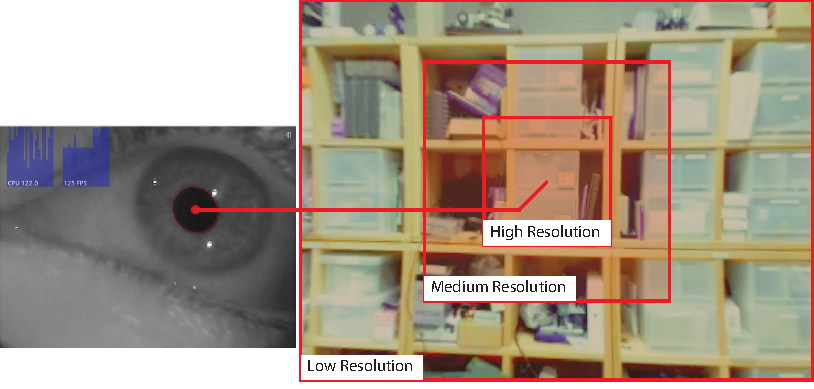
\includegraphics[width=1\linewidth]{figures/system/Foveation.pdf}
\centering
  \captionsetup{justification=centering}
\caption{Foveated Streaming overview: multi-resolution regions based on eye gaze position.}
\label{fig.intro}
\end{figure}

\subsection{Foveated Streaming}

To address the previous issues related to Telexistence and Telepresence systems, a perceptual driven approach was used. Human eyes have the highest visual acuity at the fovea in the retina, which is only about $2\deg$ of the visual field, and this visual acuity decreases the further it is from the center of the fovea towards the peripheral vision. By taking the advantages of this property, a multi-resolution image stream is generated from the original high-resolution images of the Teleoperated system. This multi-resolution stream maintains the high visual quality at the center of the eye gaze, while lower spatial resolution images are used for the peripheral area as shown in Figure \ref{fig.intro}. Using this method, the image stream would result in a higher compression ratio based on the selected fovea size, and the encoding/decoding performance would increase according to that too. This paper is based on the previous research area of foveated rendering, and it contributes as follows:
\begin{itemize}
\item Providing real-time network streaming synchronization for eye-gaze using RTP stream.
\item Quantitative and qualitative studies showing the effect of foveated streaming for performance and human perception.
%\item Extending the method for equirectangular  image streaming.
\end{itemize} 

The idea of using eye fovea as a driver to optimize the image spatial resolution has developed an important body of research in the area of multimedia and computer graphics optimization. In image compression, Wang et al. \cite{wang2001embedded} proposed image coding system by taking into consideration the nonlinear decrease of spatial resolution in the human eye, and removing the high-frequency information from the peripheral area, thus improving the overall compression performance. Itti \cite{itti2004automatic} used a different approach to address image compression by using saliency information rather than just the eye gaze position. And Ryoo et al. \cite{ryoo2016design} proposed a video streaming service based on eye gaze foveation to enhance network bandwidth. In computer graphics, Guenter et al. \cite{guenter2012foveated} used foveated rendering in order to enhance rendering performance by 5-6 times than direct rendering. Patney et al. \cite{patney2016perceptually} used foveated rendering in virtual reality applications to reduce the rendering cost, the work showed that foveated rendering did not introduce a significant difference in visual quality compared to direct rendering.


\subsection{Encoding \& Streaming}

Foveated streaming pipeline is shown in Figure \ref{fig.system}. This pipeline runs on the robot side, and the eye-gaze data is received from the user side. The pipeline generates a number of regions (N) which can be set in using system parameters. Region size in degrees is also determined by the Fovea Size parameter, in the conducted experiments, a value of 15 deg produced a good balance between streaming compression and perceptual awareness. The generated regions are combined into a single image frame as in Figure \ref{fig.levels} (Streamed Regions). Then the images are compressed using the H264 encoder and converted to RTP stream to be sent to the user side. One important thing is to synchronize the eye gaze information in order to reproduce the same arrangements when combining the images on the user side. To do that, eye gaze information used for foveation is embedded into the first RTP packet of the image frame before being sent to the user. The main advantage of embedding this information into the RTP stream is to ensure exact synchronization of the data and the image stream when rebuilding the original image at the user side.

\subsection{Unpacking \& Presentation}

User side receives the packed regions as an image stream, each frame contains foveation levels as was described in the previous section. When decoding the stream,  first the eye gaze position is extracted from the first RTP packet of the packed frame and is used to arrange the regions and positioning them exactly as they were sent. After unpacking the images, the regions are presented starting from the last region. Region number N is rendered into an offscreen image covering the entire field of view, next Region number N-1 is rendered at the original scale, and so on until Region 1 is rendered on top of them as shown in Figure \ref{fig.levels} (Foveated Image). To mitigate the effect of change in resolution between two consecutive regions, a mask is applied to each region which helps to fade the edges and to reproduce similar effect of eye retina decrease of visual acuity, while maintaining high resolution at the center of the region as shown in Figure \ref{fig.levels} (Region Masking).

\begin{figure} [t!]
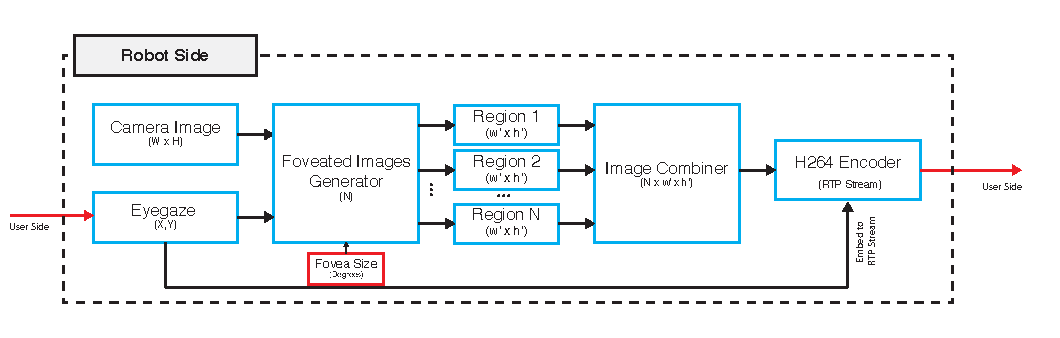
\includegraphics[width=1\linewidth]{figures/system/fov-system.pdf}
\centering
  \captionsetup{justification=centering}
\caption{Foveated Streaming pipeline.}
\label{fig.system}
\end{figure}


\begin{figure} [t!]
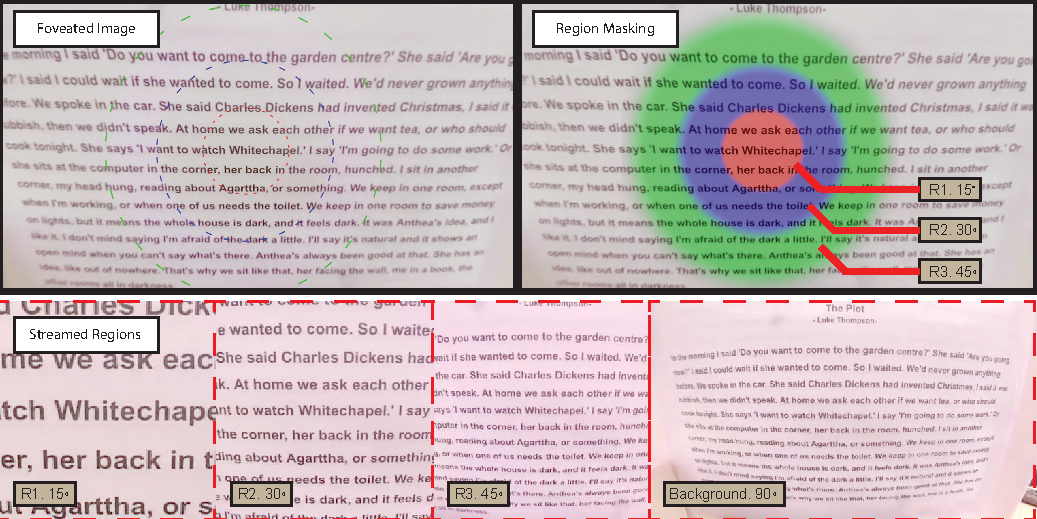
\includegraphics[width=1\linewidth]{figures/system/FoveationLevels.pdf}
\centering
  \captionsetup{justification=centering}
\caption{Foveated streaming decomposition (1) Foveated Image: final reproduced image at the user side, (2) Region Masking: masks used for combining the regions, and (3) Streamed Regions: streamed frame containing regions of foveation.}
\label{fig.levels}
\end{figure}


\subsection{Evaluation}
To evaluate foveated streaming method, two types of evaluation were conducted:
\begin{itemize}
\item Performance Evaluation: to evaluate the overall performance of the system compared with full resolution image streaming, the bandwidth usage, and CPU consumption are tested.
\item Qualitative Evaluation: a user study confirming the effectiveness of foveated streaming in maintaining the perceptual consistency of visual information.
\end{itemize}

Same system and hardware setup were used in both evaluations. USB3.0 camera module (Model no. See3CAM CU130 by e-consystems) were used to capture image stream, and connected to Intel NUC for video encoding and streaming over an Ethernet LAN to the user side. For media encoding and streaming, GStreamer library was used. The video stream is compressed using H.264 video codec provided by the library.

\subsubsection{Performance Evaluation}
The goal of performance evaluation is to measure the effectiveness of using foveated streaming network bandwidth, and CPU performance at the encoder side compared with full resolution streaming. In this evaluation, three different streaming modes were used: 640x480 pixels at 60 FPS, 1280x720 pixels at 60 FPS, and 1920x1080 pixels at 30 FPS. To maintain image quality among the images in both cases, adaptive bitrate quantizer set at 20\% was used for the video codec. Foveated streaming parameters used were: $15\deg$ Fovea Size, and 3 levels of foveation.  Figure \ref{fig.PerfEval} shows the quantitative results the proposed system. The results show the performance effectiveness of foveated streaming compared to full resolution streaming for both the bandwidth (compression rate varies from 5 to 8 depending on the streaming resolution) and CPU load (about half CPU usage for foveated streaming). 

\begin{figure} [t!]
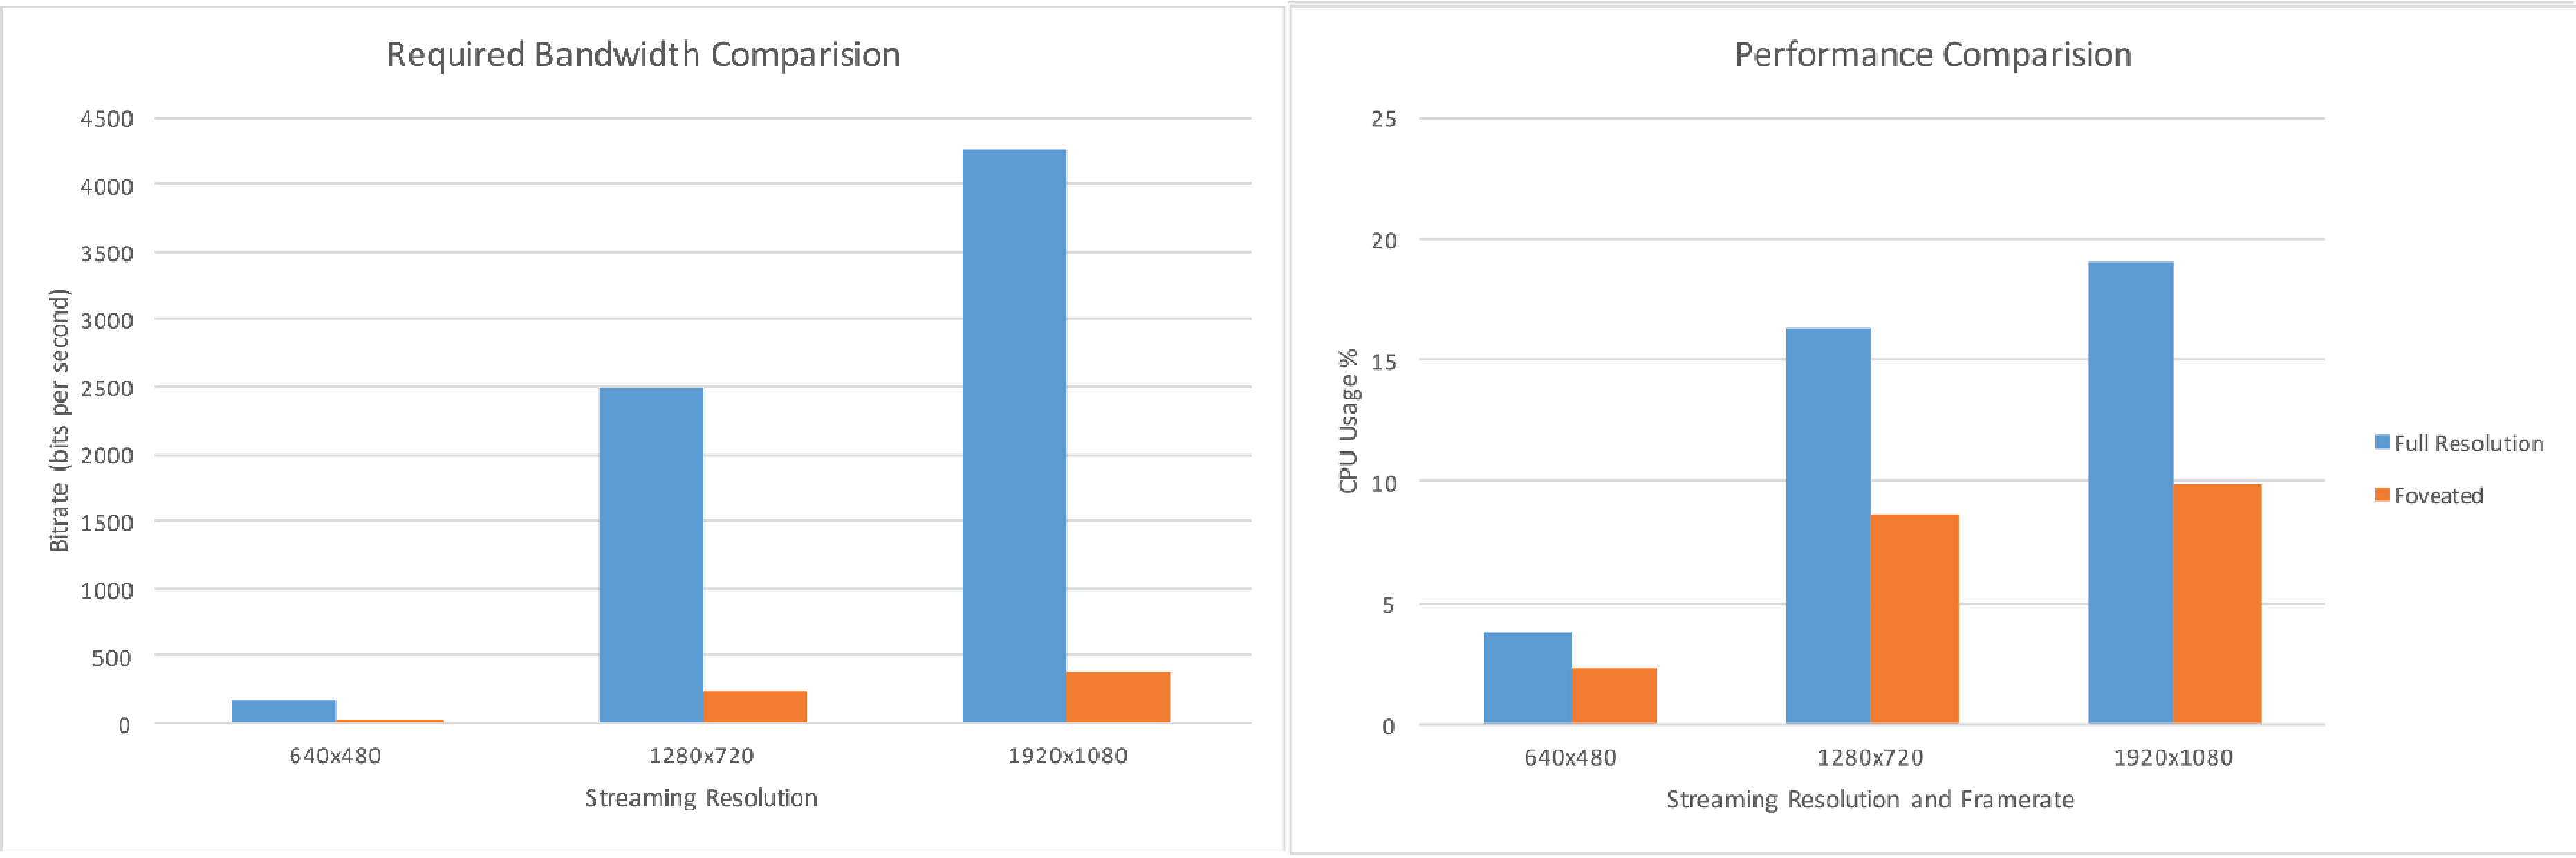
\includegraphics[width=1\linewidth]{figures/system/fov-Eval1.pdf}
\centering
  \captionsetup{justification=centering}
\caption{Performance evaluation of foveated streaming compared with full resolution streaming.}
\label{fig.PerfEval}
\end{figure}


\subsubsection{Qualitative Evaluation}
A user study was conducted to evaluate the visual perceptual effectiveness when using foveated streaming compared to full resolution streaming. The hypothesis is when using foveated streaming, there is no significant difference in reading speed compared when using full resolution streaming. 

The study setup consisted of a three-axis telexistence robot head (providing pitch, yaw, roll motion) equipped with $90\deg$ cameras for video streaming. The cameras were set to capture 1920x1080 pixels at 30 FPS when streaming. For foveated streaming settings, fovea size used was $15\deg$ with 3 levels of foveation resulting a stream of 1528x320 pixels per image. An A3 paper containing one page of text (font used bold Arial at a font size of 24points, and 1.5 line spacing) placed in front of the robot at a distance of 30cm. Page was fixed that the first line of text is placed at the eye level of the robot. The total number of pages is 5, with an average of 225 words per page. The text used was a short English essay (The Plot by Luke Thompson). The user is connected to the robot over the network and uses an HMD to control the head motion of the robot and to perceive the visual information from it. The HMD is equipped with an eye gaze tracker (Pupil-lab for Oculus DK2) to measure eye movement when the foveated streaming mode is enabled. In this setup, the user will be required to use both his head motion and eye motion to read the text from the beginning to the end of the page along yaw and pitch axes. 


\begin{figure} [hpbt]
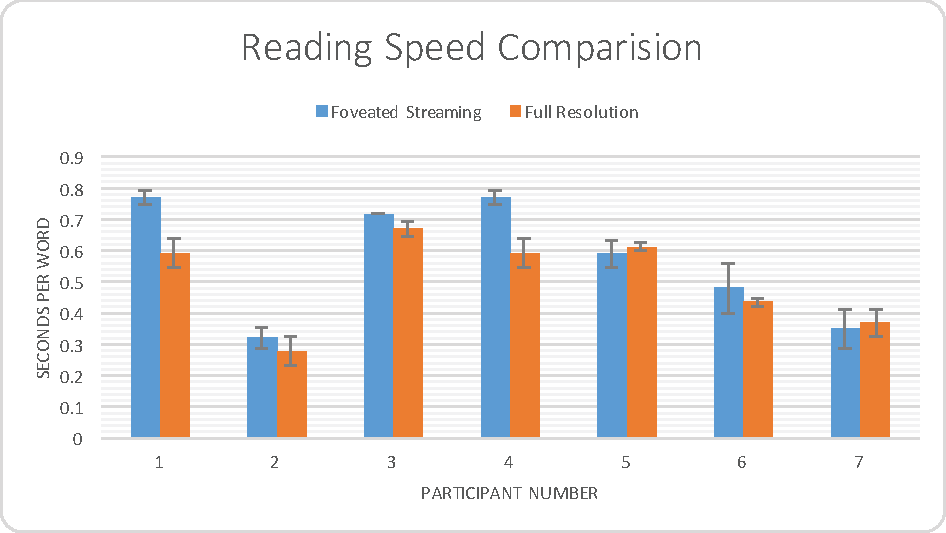
\includegraphics[width=1\linewidth]{figures/system/fov-UserEval.pdf}
\centering
  \captionsetup{justification=centering}
\caption{Subjective evaluation of reading speed for foveated streaming and full resolution streaming.}
\label{fig.UserEval}
\end{figure}


Prior to the study, participants are asked to fill a questionnaire containing basic information such as the age, eyes visual acuity for the left and right eye, and frequency of using HMDs in general. The participants are only informed of the task of reading an essay at one page a time and were asked to inform the experimenter once they finished reading the active page. After wearing the HMD, the participants are asked to calibrate their eye gaze using 9-points eye gaze calibration procedure, then a waiting gray screen is shown before starting reading. Once they inform their readiness to start reading, the user gets connected to the robot, and they start reading the text from top to bottom, left to right. After reading the page is finished, the waiting screen is shown again and the procedure continues to the next page until the 5 pages are over. The streaming mode for the pages is switched between full streaming/foveated streaming when changing the pages, and the first page's mode is randomly selected between both modes. Reading time is measured per page and stored along with the streaming mode for performance evaluation. After the study is over, qualitative questions are asked about the reading experience and whether anything has been noticed while reading and switching the pages.  

 In this evaluation, 7 participants joined the study (6 males and 1 female with an average age of $24\pm 3$) from different ethnicities. Overall feedback did not include any significant difference in the reading experience of the pages. Two participants reported seeing blurry words around the edges of gaze point (participant 1 and 4), this is due to the eye gaze tracker which could have been moved during the experiments (HMD was moved from the calibration position), the performance results show the impact of the calibration mismatch to their reading speed in foveated streaming. For performance results of the study, Figure \ref{fig.UserEval} shows the average time per word for both full resolution and foveated streaming per participant. Overall reading speed can of both modes shows no significant difference between both modes. Reading speed varies per page, and overall the speed slightly increases when proceeding in the study, this can be due to the adaptation time of reading over a Telexistence robot. From these results, it can be shown that foveated streaming provided similar results to the full streaming under the condition of consistent eye gaze tracking.
